%============================================================
%  Claremont McKenna College — Senior Thesis
%  Computational biology
%============================================================

\documentclass[12pt, oneside]{report}

%------------------------------------------------------------
% Packages
%------------------------------------------------------------
\usepackage[margin=1in]{geometry}
\usepackage{setspace}
\usepackage{times}           % Times New Roman equivalent
\usepackage{microtype}       % better line-breaking
\usepackage{amsmath}
\usepackage{amssymb}
\usepackage{graphicx}
\usepackage{float}
\usepackage{caption}
\usepackage{subcaption}
\usepackage{booktabs}        % professional tables
\usepackage{array}
\usepackage{longtable}
\usepackage{tabularx}
\usepackage{multirow}
\usepackage{hyperref}
\usepackage[super,comma,sort]{natbib}   % superscript numbered citations
\usepackage{titlesec}        % section heading formatting
\usepackage{tocloft}         % TOC formatting
\usepackage{fancyhdr}        % headers/footers
\usepackage{emptypage}       % suppress headers on blank pages
\usepackage{indentfirst}     % indent first paragraph of each section
\usepackage{parskip}         % space between paragraphs when no indent desired
\usepackage[utf8]{inputenc}
\usepackage[T1]{fontenc}
%\usepackage{lmodern}  % not available in this environment

%------------------------------------------------------------
% Page layout
%------------------------------------------------------------
\geometry{
  top    = 1.0in,
  bottom = 1.0in,
  left   = 1.25in,
  right  = 1.0in
}

\doublespacing

%------------------------------------------------------------
% Header / footer
%------------------------------------------------------------
\pagestyle{fancy}
\fancyhf{}
\renewcommand{\headrulewidth}{0.4pt}
\fancyhead[R]{\thepage}
\fancyhead[L]{\leftmark}

\fancypagestyle{plain}{%
  \fancyhf{}
  \renewcommand{\headrulewidth}{0pt}
  \fancyfoot[C]{\thepage}
}

%------------------------------------------------------------
% Section heading styles
%------------------------------------------------------------
\titleformat{\chapter}[display]
  {\normalfont\large\bfseries\centering}
  {\chaptertitlename\ \thechapter}{10pt}{\large}

\titleformat{\section}
  {\normalfont\normalsize\bfseries}
  {\thesection}{1em}{}

\titleformat{\subsection}
  {\normalfont\normalsize\itshape}
  {\thesubsection}{1em}{}

%------------------------------------------------------------
% Caption formatting
%------------------------------------------------------------
\captionsetup{
  font       = small,
  labelfont  = bf,
  format     = plain,
  justification = raggedright,
  singlelinecheck = false
}

%------------------------------------------------------------
% Hyperref setup (no coloured boxes)
%------------------------------------------------------------
\hypersetup{
  colorlinks = true,
  linkcolor  = black,
  citecolor  = black,
  urlcolor   = black
}

%------------------------------------------------------------
% Custom commands
%------------------------------------------------------------
\newcommand{\figplaceholder}[2]{%
  \begin{figure}[H]
    \centering
    \fbox{\parbox{0.85\textwidth}{%
      \centering\vspace{2cm}
      \textit{[Figure #1: #2]}
      \vspace{2cm}
    }}
    \caption{#2}
    \label{fig:#1}
  \end{figure}
}

%============================================================
\begin{document}
%============================================================

%------------------------------------------------------------
%------------------------------------------------------------
%------------------------------------------------------------
% TITLE PAGE
%------------------------------------------------------------
\begin{titlepage}
  \centering
  \vspace*{1.5in}
  {\Large\bfseries
    Title
  }\par
  \vspace{1.0in}
  {\normalsize A Thesis Presented by}\par
  \vspace{0.3in}
  {\large Matthew Jabro}\par
  \vspace{0.3in}
  {\normalsize To\\[0.3em]
  Claremont McKenna College}\par
  \vspace{0.5in}
  {\normalsize
    In partial fulfillment of\\[0.3em]
    The degree of Bachelor of Arts\\[0.3em]
    Senior Thesis in Data Science
  }\par
  \vspace{0.5in}
  {\normalsize Reader: Professor Shibu Yooseph}\par
  \vfill
  {\normalsize May 2026}
\end{titlepage}

%------------------------------------------------------------
% FRONT MATTER (roman numerals)
%------------------------------------------------------------
\pagenumbering{roman}
\setcounter{page}{2}

%--- Acknowledgements ---------------------------------------
\chapter*{Acknowledgements}
\addcontentsline{toc}{chapter}{Acknowledgements}

This material is based upon work supported by the National Science Foundation under Award
No.\ 2408259. [Add any additional acknowledgements here.]

\newpage

%--- Abstract -----------------------------------------------
\chapter*{Abstract}
\addcontentsline{toc}{chapter}{Abstract}

[Abstract text to be inserted here.]

\newpage

%--- Table of Contents --------------------------------------
\tableofcontents
\newpage

%--- List of Figures ----------------------------------------
\listoffigures
\addcontentsline{toc}{chapter}{List of Figures}
\newpage

%--- List of Tables -----------------------------------------
\listoftables
\addcontentsline{toc}{chapter}{List of Tables}
\newpage

%------------------------------------------------------------
% MAIN MATTER (arabic numerals)
%------------------------------------------------------------
\pagenumbering{arabic}
\setcounter{page}{1}

%============================================================
\chapter{Introduction}
%============================================================

Soil is among the most microbially diverse environments on Earth. A single gram can
harbor thousands of distinct bacterial taxa, and the collective activity of these communities
drives the biogeochemical cycles that underpin terrestrial ecosystem function globally
(Fierer et al.\ 2006). Despite this importance, large-scale patterns in soil microbial
community structure remain difficult to characterize: whether predictable community types
exist across biomes and whether composition encodes the environment of origin remain open
questions at global scale.

Two DNA sequencing strategies exist for profiling these communities. Shotgun
metagenomics sequences DNA extracted from a soil sample, providing both functional and
taxonomic information but at increased cost and computational burden that limits the total
number of samples that can be sequenced. 16S ribosomal RNA (rRNA) amplicon sequencing
offers a complementary approach. Because the 16S gene is phylogenetically conserved across
all bacteria and archaea yet contains hypervariable regions sufficient to discriminate taxa, it
allows community-wide profiling at taxonomic resolution sufficient to reach genus and family
level for most groups.

This thesis analyzes two independent global soil datasets. The first is the global topsoil
survey of Bahram et al.\ (2018), comprising 193 samples after filtering, processed from raw
FASTQ files through a DADA2 pipeline. The second is the Earth Microbiome Project (EMP)
soil subset (Thompson et al.\ 2017), comprising 2,209 samples drawn from a coordinated
multi-study archive. The datasets differ in scope, sequencing depth, and upstream processing
methodology; consistent findings in both indicate that results are robust to these differences.

We ask two questions. First, can unsupervised clustering of centered log-ratio
(CLR)-transformed profiles reveal recurring community types without reference to sample
metadata? Second, does community composition allow a random forest classifier, trained on
biome labels, to predict habitat of origin, and which taxa carry the most predictive signal?

%============================================================
\chapter{Datasets and Computational Environment}
%============================================================

%------------------------------------------------------------
\section{Global Topsoil Dataset (Bahram et al.\ 2018)}
%------------------------------------------------------------

The global topsoil dataset originates from Bahram et al.\ (2018, \textit{Nature}), a
coordinated single-survey design in which composite soil cores were collected from 189 sites
spanning all major terrestrial biomes globally, producing 7,560 subsamples with matched
environmental metadata. The bacterial 16S rRNA gene V4 region was amplified using primers
515F/806RB and sequenced on Illumina platforms as paired-end reads; raw sequence data are
publicly archived under EBI accession PRJEB19856 (ERP021922) as paired-end FASTQ files.
A total of 234 paired-end samples were downloaded for processing; 193 remained after
quality-based sample exclusions. Matched sample metadata, obtained from the SRA run table
(\texttt{sraRunTable.csv}), include biome type, country of collection, geographic coordinates
(latitude and longitude), elevation, soil pH, and mean annual temperature. For classification
analyses, the original biome categories were consolidated into seven broader groups (see
Section~\ref{sec:biome-grouping}). After prevalence filtering and CLR transformation, the final
feature matrix contains 193 samples~$\times$~165 genus-level lineages.

%------------------------------------------------------------
\section{EMP Soil Subset (Thompson et al.\ 2017)}
%------------------------------------------------------------

The Earth Microbiome Project (EMP) dataset originates from Thompson et al.\
(2017, \textit{Nature}), which aggregated and harmonized 16S rRNA amplicon data from
97 independent studies comprising 27,751 samples spanning diverse environment types
worldwide. EMP Release 1 data were obtained from Zenodo as three files: the Deblur count
table (\texttt{emp\_deblur\_150bp\_release1.biom}), a representative FASTA file of all unique
sequences (\texttt{emp\_deblur\_150bp\_min25.fasta}), and the comprehensive metadata table
(\texttt{emp\_metadata\_release1\_20170912.tsv}). Soil samples were extracted by filtering on
the \texttt{env\_material} metadata field using the regular expression
\texttt{soil|sediment|rhizosphere}, yielding 2,209 samples. Available metadata include Earth
Microbiome Project Ontology (EMPO) environment classification at three hierarchical levels,
Environmental Ontology (ENVO) biome descriptors at four levels, and continuous
physicochemical measurements including pH, temperature, salinity, phosphate, nitrate,
ammonium, elevation, and geographic coordinates. For classification analyses, biome
annotations were consolidated into a 10-group scheme (see Section~\ref{sec:biome-grouping}).
After prevalence filtering and CLR transformation, the final feature matrix contains
2,209 samples~$\times$~1,533 genus-level lineages.

%------------------------------------------------------------
\section{Dataset Comparison}
%------------------------------------------------------------

Table~\ref{tab:dataset-comparison} summarizes the key design and processing differences
between the two datasets.

\begin{table}[H]
\centering
\caption{Comparison of the two soil microbiome datasets analyzed in this thesis.}
\label{tab:dataset-comparison}
\small
\begin{tabularx}{\textwidth}{l X X}
\toprule
& \textbf{Global Topsoil (Bahram et al.\ 2018)} & \textbf{EMP Soil Subset (Thompson et al.\ 2017)} \\
\midrule
Study Design
  & Single coordinated survey
  & Multi-study meta-analysis (97 independent studies) \\[4pt]
Original Scope
  & 189 sites; 7,560 subsamples across all major terrestrial biomes
  & 27,751 samples across diverse global environments; soil subset extracted \\[4pt]
Samples Analyzed
  & 193 (after quality-based exclusions)
  & 2,209 (filtered on \texttt{env\_material}: soil, sediment, rhizosphere) \\[4pt]
Target Region
  & 16S rRNA V4 (primers 515F/806RB)
  & 16S rRNA V4 (primers 515F/806RB) \\[4pt]
Read Processing
  & Raw FASTQ reprocessed here via DADA2 v1.26.0 pipeline
  & Pre-processed centrally by EMP using Deblur at fixed 150 bp truncation;
    obtained as release BIOM table \\[4pt]
Taxonomy Reference
  & SILVA v138.2, genus level
  & SILVA v138.1, genus level (assigned \textit{de novo} from representative FASTA) \\[4pt]
Environmental Metadata
  & Biome type, country, latitude/longitude, elevation, soil pH,
    mean annual temperature
  & EMPO classification (3 hierarchical levels), ENVO biome descriptors
    (4 levels), pH, temperature, salinity, phosphate, nitrate, ammonium,
    elevation, coordinates \\[4pt]
Access
  & Raw FASTQ; EBI accession PRJEB19856 (ERP021922)
  & Pre-processed BIOM table; EMP Release 1 via Zenodo
    (DOI 10.5281/zenodo.890000) \\
\bottomrule
\end{tabularx}
\end{table}

%------------------------------------------------------------
\section{Computational Environment}
%------------------------------------------------------------

All analyses were performed on the Hopper high performance computer (HPC) cluster at
Claremont McKenna College (Rocky Linux), managed by SLURM. Compute nodes provide up to
128 CPUs and either 750 GB RAM or 3 TB RAM (high-memory nodes). Each analytical step is
wrapped in a dedicated SLURM batch script and output files from each step are written to
structured subdirectories to ensure reproducibility and auditability of the full pipeline.

R 4.2.0 (deployed via a dedicated \texttt{r-dada2} conda environment) was the primary
language throughout, with the following packages providing core functionality: DADA2
(Callahan et al.\ 2016)\cite{callahan2016} for amplicon denoising; Biostrings and phyloseq
(McMurdie et al.\ 2013)\cite{mcmurdie2013} for sequence and count-table handling; vegan
(Dixon 2003)\cite{dixon2003} for alpha diversity metrics; randomForest (Breiman
2001)\cite{breiman2001} and caret for classifier training and train/test partitioning; Rtsne
(van der Maaten and Hinton 2008)\cite{maaten2008} for non-linear dimensionality reduction;
pheatmap and ggplot2 for visualization; and tidyverse for data manipulation throughout.
Cluster metadata visualization was implemented in Python using pandas, seaborn, and
matplotlib.

%============================================================
\chapter{Methods}
%============================================================

%------------------------------------------------------------
\section{Sequence Processing — Global Topsoil (DADA2 Pipeline)}
\label{sec:dada2}
%------------------------------------------------------------

Raw paired-end FASTQ files were processed through a DADA2 amplicon sequence variant
(ASV) pipeline in R on an HPC cluster. The full pipeline structure is shown in
Figure~\ref{fig:1}; per-step read retention statistics are provided in Supplementary Table~1.
The SILVA v138.2 genus-level reference (Quast et al.\ 2013)\cite{quast2013} was pre-filtered
to remove Eukaryota, Chloroplast, and Mitochondria entries prior to taxonomy assignment.
Reads were quality-filtered with \texttt{filterAndTrim()} (maximum errors set to 2, minimum
quality cutoff Q\,=\,2). Sequencing error models were estimated independently for forward and
reverse reads with \texttt{learnErrors()}, and denoising was performed with \texttt{dada()}.
Denoised reads were merged with \texttt{mergePairs()}, and samples with inadequate overlap
were excluded. An ASV count matrix was constructed with \texttt{makeSequenceTable()} and
chimeric sequences removed with \texttt{removeBimeraDenovo()}. Non-bacterial ASVs
(chloroplasts, mitochondria, eukaryotic 18S) were removed, and per-sample read counts were
tracked across all stages as a quality-control (QC) check.

Taxonomy was assigned against the pre-filtered SILVA v138.2 reference to genus level
with \texttt{assignTaxonomy()}. Lineages present in fewer than 20 of 193 samples were
excluded. The centered log-ratio (CLR) transformation (Aitchison 1986)\cite{aitchison1986}
was then applied, producing the final feature matrix.

%--- Figure 1 placeholder -----------------------------------
\begin{figure}[H]
  \centering
  
\includegraphics[width=0.42\linewidth]{Fig1_Thesis.png}
    \caption[DADA2 processing pipeline — Global Topsoil Dataset]{
    DADA2 processing pipeline for the global topsoil dataset (Bahram et al.\ 2018),
    run on EBI accession PRJEB19856. Steps proceed top to bottom: classifier
    filtering (SILVA v138.2; Eukaryota, Chloroplast, and Mitochondria removed),
    quality filtering (\texttt{filterAndTrim()}; 77\% retained), error rate learning
    (\texttt{learnErrors()}), denoising (\texttt{dada()}), paired-end merging
    (\texttt{mergePairs()}; 43.7\% retained), ASV table construction
    (\texttt{makeSequenceTable()}; 33.3\% retained), eukaryote removal, ASV
    tracking (exported as QC), taxonomy assignment (\texttt{assignTaxonomy()};
    resolved to genus level), and CLR transformation (lineages present in
    $\geq$\,20 of 193 samples retained; final feature matrix produced).
    Individual scripts (Script 00–09) correspond to each step and are provided
    as supplementary materials.
  }
  \label{fig:1}
\end{figure}

%------------------------------------------------------------
\section{Sequence Processing — EMP Soil Subset}
\label{sec:emp-processing}
%------------------------------------------------------------

The EMP soil subset was obtained from the EMP Release 1 Zenodo archive
(DOI 10.5281/zenodo.890000) as a pre-processed resource. The data released included a
centrally harmonized ASV table denoised with Deblur (Amir et al.\ 2017)\cite{amir2017} at a
fixed 150 bp read length, accompanied by a representative FASTA file of all unique sequences
and a comprehensive metadata table. The full processing pipeline is shown in
Figure~\ref{fig:2}; key statistics are provided in Supplementary Table~2.

Soil samples were extracted by filtering the metadata on \texttt{env\_material} using the
regular expression \texttt{soil|sediment|rhizosphere}. The BIOM count table was converted to
TSV with \texttt{biom convert} and parsed in R to a dense ASV~$\times$~sample matrix.
Because the EMP release uses internal sequence identifiers rather than taxonomy strings,
taxonomy was assigned \textit{de novo} with the SILVA v138.1 genus-level reference. ASV-level
counts were then collapsed to genus level by summing counts sharing a resolved genus
assignment; entries with unresolved (NA) genus were discarded. Samples present in the
metadata but absent from the Deblur count matrix were inserted as all-zero rows.

%--- Figure 2 placeholder -----------------------------------
\begin{figure}[H]
  \centering
  
\includegraphics[width=0.5\linewidth]{Fig2_Thesis_(1).png}  
    \caption[Processing pipeline — EMP Soil Subset]{
    Processing pipeline for the EMP soil subset (Thompson et al.\ 2017). Entry
    point is the EMP Release 1 archive (Deblur ASV table and representative FASTA).
    Steps: soil sample extraction (env\_material filtered for soil, sediment, and
    rhizosphere), BIOM parse/count matrix construction (\texttt{biom convert}
    $\rightarrow$ TSV; ASV\,$\times$\,sample matrix), taxonomy assignment
    (\texttt{assignTaxonomy()}; genus level), genus-level collapse (ASV counts summed
    by genus; NA entries discarded), quality control (richness distributions; count
    vs.\ genus cross-check), prevalence filtering (threshold selection via sweep), and
    CLR transformation (per-sample log-ratio applied; final feature matrix produced).
    Individual scripts (Script 10–16) are provided as supplementary materials.
  }
  \label{fig:2}
\end{figure}

%------------------------------------------------------------
\section{Quality Control}
\label{sec:qc}
%------------------------------------------------------------

For the global topsoil dataset, per-sample ASV richness was computed directly from the
post-chimera DADA2 object. Row sums and per-sample genus richness of the genus-collapsed
matrix were also computed and exported. Read counts through all DADA2 stages were tracked.

For the EMP dataset, a read count vs.\ genus count comparison verified that
genus-collapsed counts summed consistently with raw read totals. A cross-reference check
confirmed that all ASV identifiers in the representative FASTA, taxonomy table, and count
matrix were mutually consistent.

%------------------------------------------------------------
\section{Prevalence Filtering and Threshold Analysis}
\label{sec:prevalence}
%------------------------------------------------------------

A prevalence filter was applied to both datasets prior to CLR transformation to reduce
dimensionality while preserving compositional signal. A sweep over minimum-prevalence values
was performed for each dataset, computing at each cutoff the fraction of lineages retained and
the fraction of total abundance signal retained. A threshold of 20 samples was selected for the
global topsoil dataset, and 50 for the EMP dataset.

%------------------------------------------------------------
\section{CLR Matrix Construction}
\label{sec:clr}
%------------------------------------------------------------

The centered log-ratio (CLR) transformation (Aitchison 1986)\cite{aitchison1986} maps
compositional data into an unrestricted space, providing the geometrically appropriate metric
for compositional data analysis. The transformation pipeline is shown in Figure~\ref{fig:3}.

\begin{equation}
  \mathrm{CLR}(X_{ij}) = \log(X_{ij}+1) - \frac{1}{D}\sum_{i=1}^{D}\log(X_{ij}+1)
  \label{eq:clr}
\end{equation}

\noindent where $X_{ij}$ is the raw read count of lineage $i$ in sample $j$, and $D$ is the
total number of lineages (rows).

For the global topsoil dataset, the post-chimera bacteria-only ASV matrix was collapsed
to genus level, and samples with fewer than 5,000 total counts were removed. For the EMP
dataset, the genus-collapsed matrix from Section~\ref{sec:emp-processing} served as input
directly; samples with fewer than 5,000 total counts were likewise removed. In both cases,
the prevalence filter from Section~\ref{sec:prevalence} was applied, and a pseudocount of 1
was added to all entries to handle structural zeros.

%--- Figure 3 placeholder -----------------------------------
\begin{figure}[H]
  \centering
  
\includegraphics[width=1\linewidth]{Fig3_Thesis.png}      
    \caption[CLR transformation pipeline]{
    Centered log-ratio (CLR) transformation pipeline (Aitchison
    1986)\cite{aitchison1986}, applied identically to both datasets. Input: sparse
    integer count matrix (lineages\,$\times$\,samples). Steps left to right:
    pseudocount addition (+1, placeholder for count of zero); log transform
    ($\log(X_{ij}+1)$ per sample); row-centering (subtract per-sample geometric
    mean). The CLR formula is given in Equation~\ref{eq:clr}. Output: real-valued
    matrix suitable for standard multivariate methods.
  }
  \label{fig:3}
\end{figure}

%------------------------------------------------------------
\section{Gaussian Graphical Model Clustering}
\label{sec:gmm}
%------------------------------------------------------------

A mixture of Gaussian Graphical Models (MixGGM) framework (Yooseph
2022)\cite{yooseph2022} was applied to both CLR-transformed feature matrices to identify
recurring community types. The model was initialized with K\,=\,20 components as an upper
bound; components with negligible mixing coefficients become unpopulated after convergence,
so the effective number of clusters is determined by which components retain sample
assignments. For the global topsoil dataset, the model was fit using 25 random initializations
and 150 expectation-maximization (EM) iterations, retaining the solution with the highest
evidence lower bound (ELBO) across all starts. For the EMP dataset, computational constraints
required reducing the fitting procedure to 5 random initializations and 10 EM iterations. Each
sample receives a posterior probability of membership in each of the K components; hard cluster
labels were assigned by taking the argmax posterior membership probability and exported for
all downstream analyses.

%------------------------------------------------------------
\section{Cluster Characterization by Metadata}
\label{sec:cluster-char}
%------------------------------------------------------------

Cluster assignments were joined to sample metadata on sample identifiers to produce an
annotated table linking each sample's cluster label to all available environmental variables
(Supplementary Table~4). For the global topsoil dataset this included biome type, country,
geographic coordinates, elevation, soil pH, and mean annual temperature. For the EMP dataset
it included EMPO classification at three hierarchical levels, ENVO biome descriptors at four
levels, and continuous physicochemical measurements. To characterize the taxonomic signature
of each cluster, the mean CLR value for every lineage was computed across all samples assigned
to that cluster, producing a lineages\,$\times$\,clusters matrix of average CLR abundances.
Stacked bar plots of biome composition per cluster, strip plots of continuous variables by
cluster, and a lineages\,$\times$\,clusters heatmap of mean CLR values were generated. The
full pipeline for cluster characterization, alpha diversity, and enhanced CLR statistics is
shown in Figure~\ref{fig:4}.

%--- Figure 4 placeholder -----------------------------------
\begin{figure}[H]
  \centering
  
\includegraphics[width=0.9\linewidth]{Fig4_Thesis.png}
    \caption[Cluster characterization pipeline]{
    Pipeline for cluster characterization, alpha diversity analysis, and enhanced CLR
    statistics (Sections~\ref{sec:cluster-char}--\ref{sec:clr-stats}), completed twice:
    once for each dataset. Input: CLR cluster assignments (argmax posterior). Cluster
    assignments are joined to sample metadata by sample identifier, producing an annotated
    sample matrix (cluster number + environmental variables). Two parallel branches follow.
    \textit{Taxonomy branch}: mean CLR is computed per lineage across all samples in each
    cluster (lineages\,$\times$\,clusters matrix); error bar plots are produced for the top
    20 cluster-discriminatory lineages; a variance heatmap is produced for the top 50 most
    variable lineages. \textit{Environmental branch}: environmental variables are joined and
    per-variable visualizations (cluster label vs.\ environmental gradient) are generated.
  }
  \label{fig:4}
\end{figure}

%------------------------------------------------------------
\section{Alpha Diversity Analysis}
\label{sec:alpha}
%------------------------------------------------------------

Three alpha diversity metrics were computed from the bacteria-only post-chimera ASV
matrix (global topsoil) and from the genus-collapsed count matrix (EMP): observed OTUs,
Chao1 bias-corrected richness (Chao 1984)\cite{chao1984}, and Shannon entropy (Shannon
1948)\cite{shannon1948}. These were computed using the vegan package (Dixon
2003)\cite{dixon2003}. Cluster assignments were joined to the resulting per-sample table and
summary statistics (mean, SD, median, IQR) computed per cluster.

%------------------------------------------------------------
\section{Enhanced CLR Statistics per Cluster}
\label{sec:clr-stats}
%------------------------------------------------------------

For each lineage--cluster combination, four statistics were computed across all samples
assigned to that cluster: mean CLR, standard deviation, standard error, and 95\% confidence
interval. Error bar plots showing mean\,$\pm$\,95\% CI were generated for the top 20 most
cluster-discriminatory lineages (ranked by variance of cluster-mean CLR across clusters). A
variance heatmap was produced for the top 50 most variable lineages across all non-empty
clusters.

%------------------------------------------------------------
\section{Ordination}
\label{sec:ordination}
%------------------------------------------------------------

Three ordination methods were applied to the CLR matrices. Principal Component
Analysis (PCA) was performed (Pearson 1901)\cite{pearson1901} using \texttt{prcomp()} in
R, retaining 20 components. Principal Coordinate Analysis (PCoA) was computed (Gower
1966)\cite{gower1966} using \texttt{cmdscale()} and used as a consistency check; PCoA on
CLR-transformed data is mathematically equivalent to CLR-PCA. t-distributed Stochastic
Neighbor Embedding (t-SNE) was applied (van der Maaten and Hinton
2008)\cite{maaten2008} using Rtsne to capture non-linear structure not visible in linear
projections. Sample scores from all three methods were exported alongside cluster labels and
biome codes for visualization (Supplementary Table~5).

%------------------------------------------------------------
\section{Biome Grouping}
\label{sec:biome-grouping}
%------------------------------------------------------------

Specific biome annotations were consolidated into broader ecological groups prior to
classification to reduce class imbalance (Supplementary Table~5). For the global topsoil
dataset, up to 11 original biome categories were collapsed into 7 groups organized by thermal
and vegetation structure. For the EMP dataset, a 10-group scheme was applied.

%------------------------------------------------------------
\section{Random Forest Biome Classification}
\label{sec:rf}
%------------------------------------------------------------

Random forest classifiers (Breiman 2001)\cite{breiman2001} were trained on
CLR-transformed composition profiles to predict biome of origin (Supplementary Table~6).
Classes with fewer than 10 samples were excluded, and the dataset was split 70/30 into
stratified train and test sets using caret. Separate models were trained for original and grouped
biome labels, yielding four models in total. Test-set performance was assessed by accuracy,
Cohen's kappa, and macro-averaged precision, recall, and F1. Feature importance was extracted
as MeanDecreaseAccuracy (MDA) and MeanDecreaseGini for all lineages; the top 50 lineages
by permutation importance were noted.

%============================================================
\chapter{Results}
%============================================================

%------------------------------------------------------------
\section{Sequence Processing and Quality Control — Global Topsoil}
\label{res:seqproc}
%------------------------------------------------------------

A total of 234 paired-end FASTQ file pairs were downloaded from EBI accession
PRJEB19856 and processed through the DADA2 denoising pipeline. The 234 samples together
contributed 33,170,669 raw input reads. Quality filtering and primer trimming with
\texttt{filterAndTrim()} were followed by paired-end merging with \texttt{mergePairs()}.
After ASV table construction and chimeric sequence removal with
\texttt{removeBimeraDenovo()}, a mean 33.4\% of input reads were retained as non-chimeric
across all samples. Non-bacterial ASVs (chloroplasts, mitochondria, eukaryotic 18S) were
removed, and 41 samples with fewer than 5,000 non-chimeric reads were excluded as
insufficiently sequenced. The final analysis set comprised 193 samples spanning 38 countries
and latitudes from $-54.8^{\circ}$ to $78.2^{\circ}$. Per-step read counts for all samples are
provided in Supplementary Table~1. The per-sample read retention trajectory across all DADA2
stages is shown in Figure~\ref{fig:5}.

%--- Figure 5 placeholder -----------------------------------
\begin{figure}[H]
  \centering
  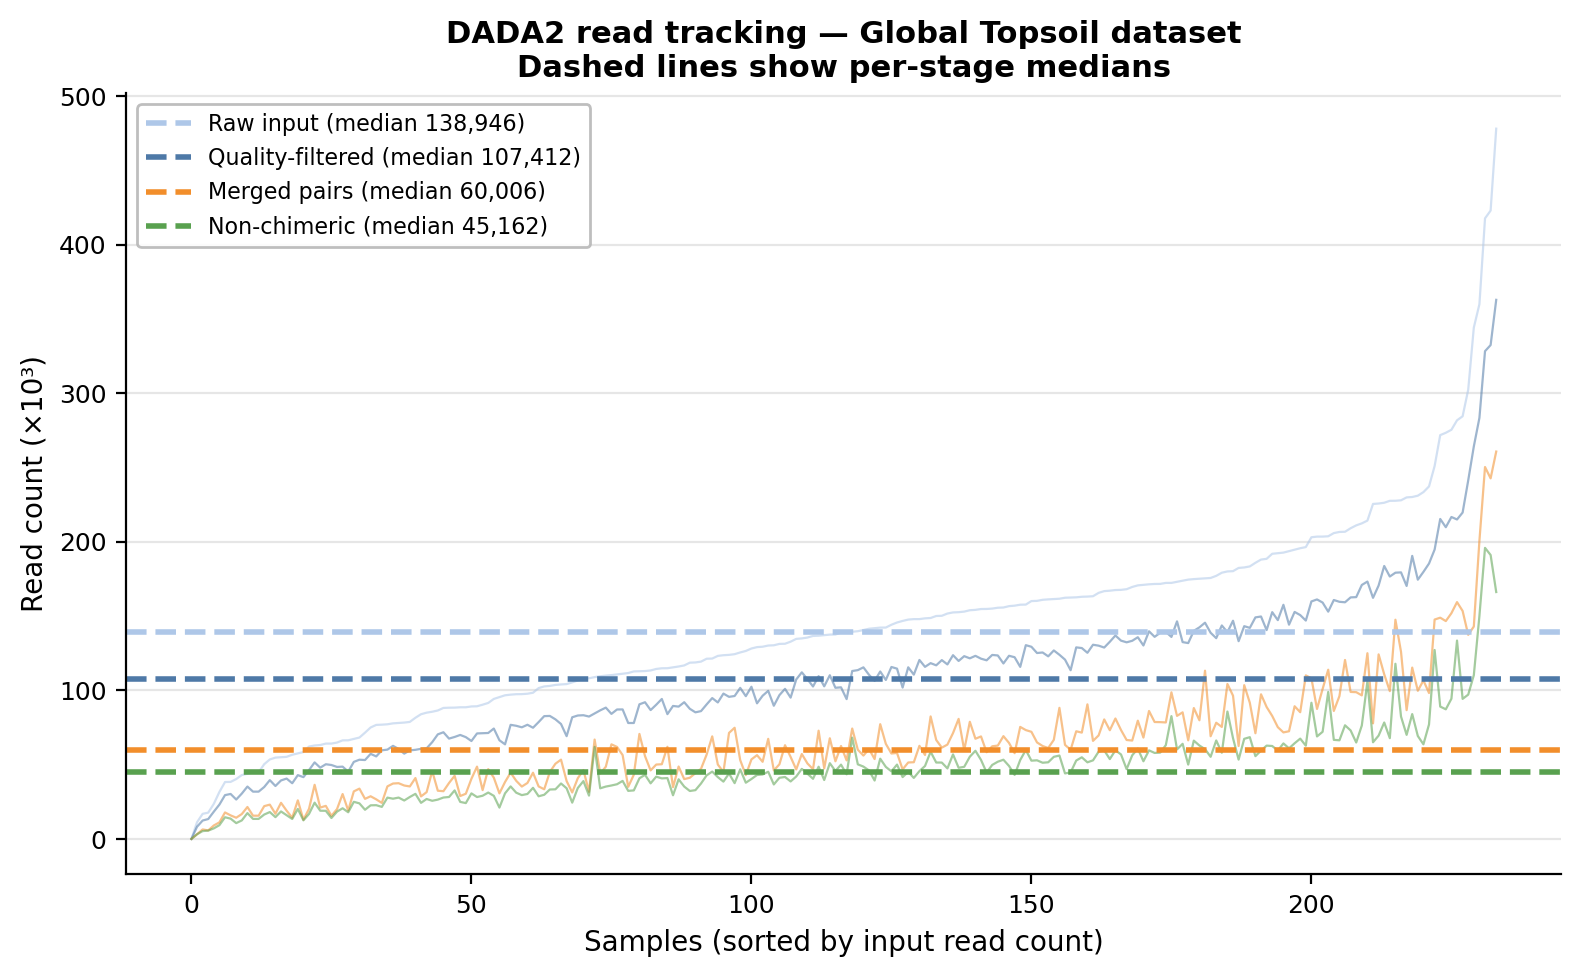
\includegraphics[width=0.9\linewidth]{fig_dada2_read_tracking.png}
    \caption[DADA2 read tracking — Global Topsoil Dataset]{
    Per-sample read retention trajectory across all DADA2 processing stages for the
    global topsoil dataset ($n\,=\,234$ samples, sorted by input read count). Dashed
    horizontal lines indicate per-stage medians: raw input (median 138,946),
    quality-filtered (median 107,412), merged pairs (median 60,006), and non-chimeric
    (median 45,162). Read counts are displayed in units of $\times 10^{3}$.
  }
  \label{fig:5}
\end{figure}

%------------------------------------------------------------
\section{Prevalence Filtering and Feature Retention}
\label{res:prevalence}
%------------------------------------------------------------

Prior to CLR transformation, genus-level lineages present in fewer than a minimum
number of samples were removed to reduce noise and dimensionality. Threshold sweep curves
plotting the fraction of lineages retained and the fraction of total read counts retained as a
function of minimum prevalence are shown in Figure~\ref{fig:6}.

For the global topsoil dataset, a threshold of 20 samples removed the majority of
low-prevalence lineages while preserving approximately 97.5\% of total read counts. The
threshold of 20 samples was approximately 10\% of the 193-sample dataset, and retained
165 genus-level lineages.

For the EMP soil subset, a threshold of 50 samples (approximately 2.3\% of 2,209
samples) was applied, retaining 1,533 genus-level lineages and approximately 98.7\% of
the read counts. In both datasets, abundance signal was well preserved at the selected
thresholds.

The final CLR-transformed feature matrices used in all downstream analyses were
193 samples\,$\times$\,165 lineages (global topsoil) and 2,209 samples\,$\times$\,1,533
lineages (EMP soil subset). Full threshold sweep statistics are provided in Supplementary
Table~3.

%--- Figure 6 placeholder -----------------------------------
\begin{figure}[H]
  \centering
  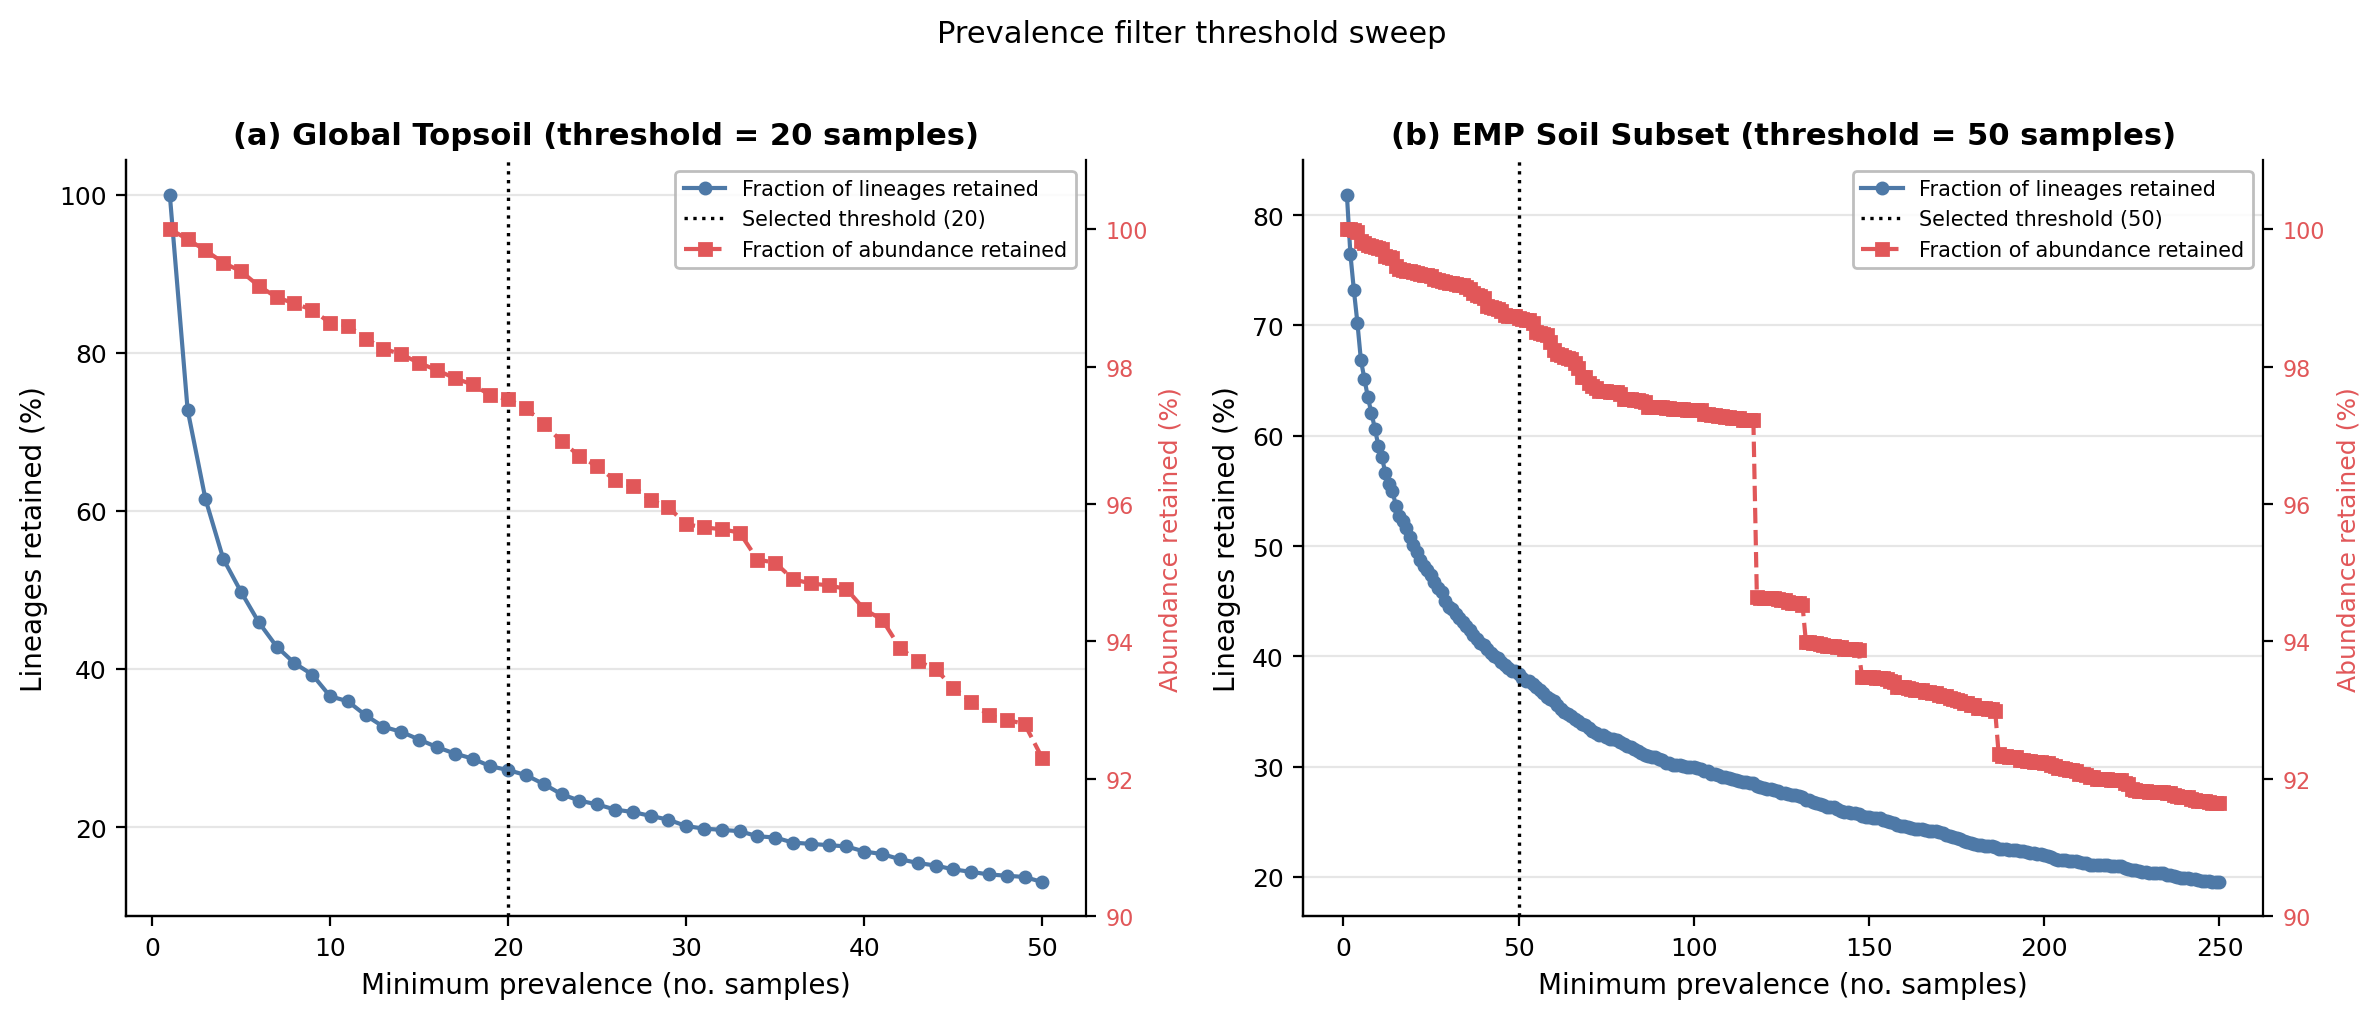
\includegraphics[width=1.05\linewidth]{fig_prevalence_sweep.png}
    \caption[Prevalence filter threshold sweep]{
    Prevalence filter threshold sweep for (a) the global topsoil dataset and (b) the
    EMP soil subset. Blue curve (left y-axis): fraction of genus-level lineages retained
    as a function of minimum prevalence threshold (number of samples). Red curve (right
    y-axis): fraction of total abundance retained. Vertical dashed lines indicate the
    selected thresholds: 20 samples for the global topsoil dataset and 50 samples for
    the EMP soil subset.
  }
  \label{fig:6}
\end{figure}

%------------------------------------------------------------
\section{MixGGM Clustering}
\label{res:gmm}
%------------------------------------------------------------

The MixGGM algorithm was applied to both CLR-transformed feature matrices to identify
recurring community types. The model was initialized with K\,=\,20 components as an upper
bound.

For the global topsoil dataset, the model was fit using 25 random initializations and
150 EM iterations, retaining the solution with the highest ELBO across all starts. After
convergence, 19 of the 20 initialized components were populated (Figure~\ref{fig:7}a).
Cluster sizes ranged from 2 to 39 samples across the 193-sample dataset. The largest
cluster was Cluster~17 ($n\,=\,39$), while Clusters~3, 4, and~7 each contained only
2 samples.

For the EMP soil subset, computational constraints imposed by the larger dataset required
reducing the fitting procedure to 5 random initializations and 10 EM iterations. Despite the
reduced search, the model converged on a solution in which only 10 of the 20 initialized
components were populated, accounting for all 2,209 samples (Figure~\ref{fig:7}b). Cluster
sizes ranged from 33 (Cluster~11) to 792 (Cluster~3).

%--- Figure 7 placeholder -----------------------------------
\begin{figure}[H]
  \centering
  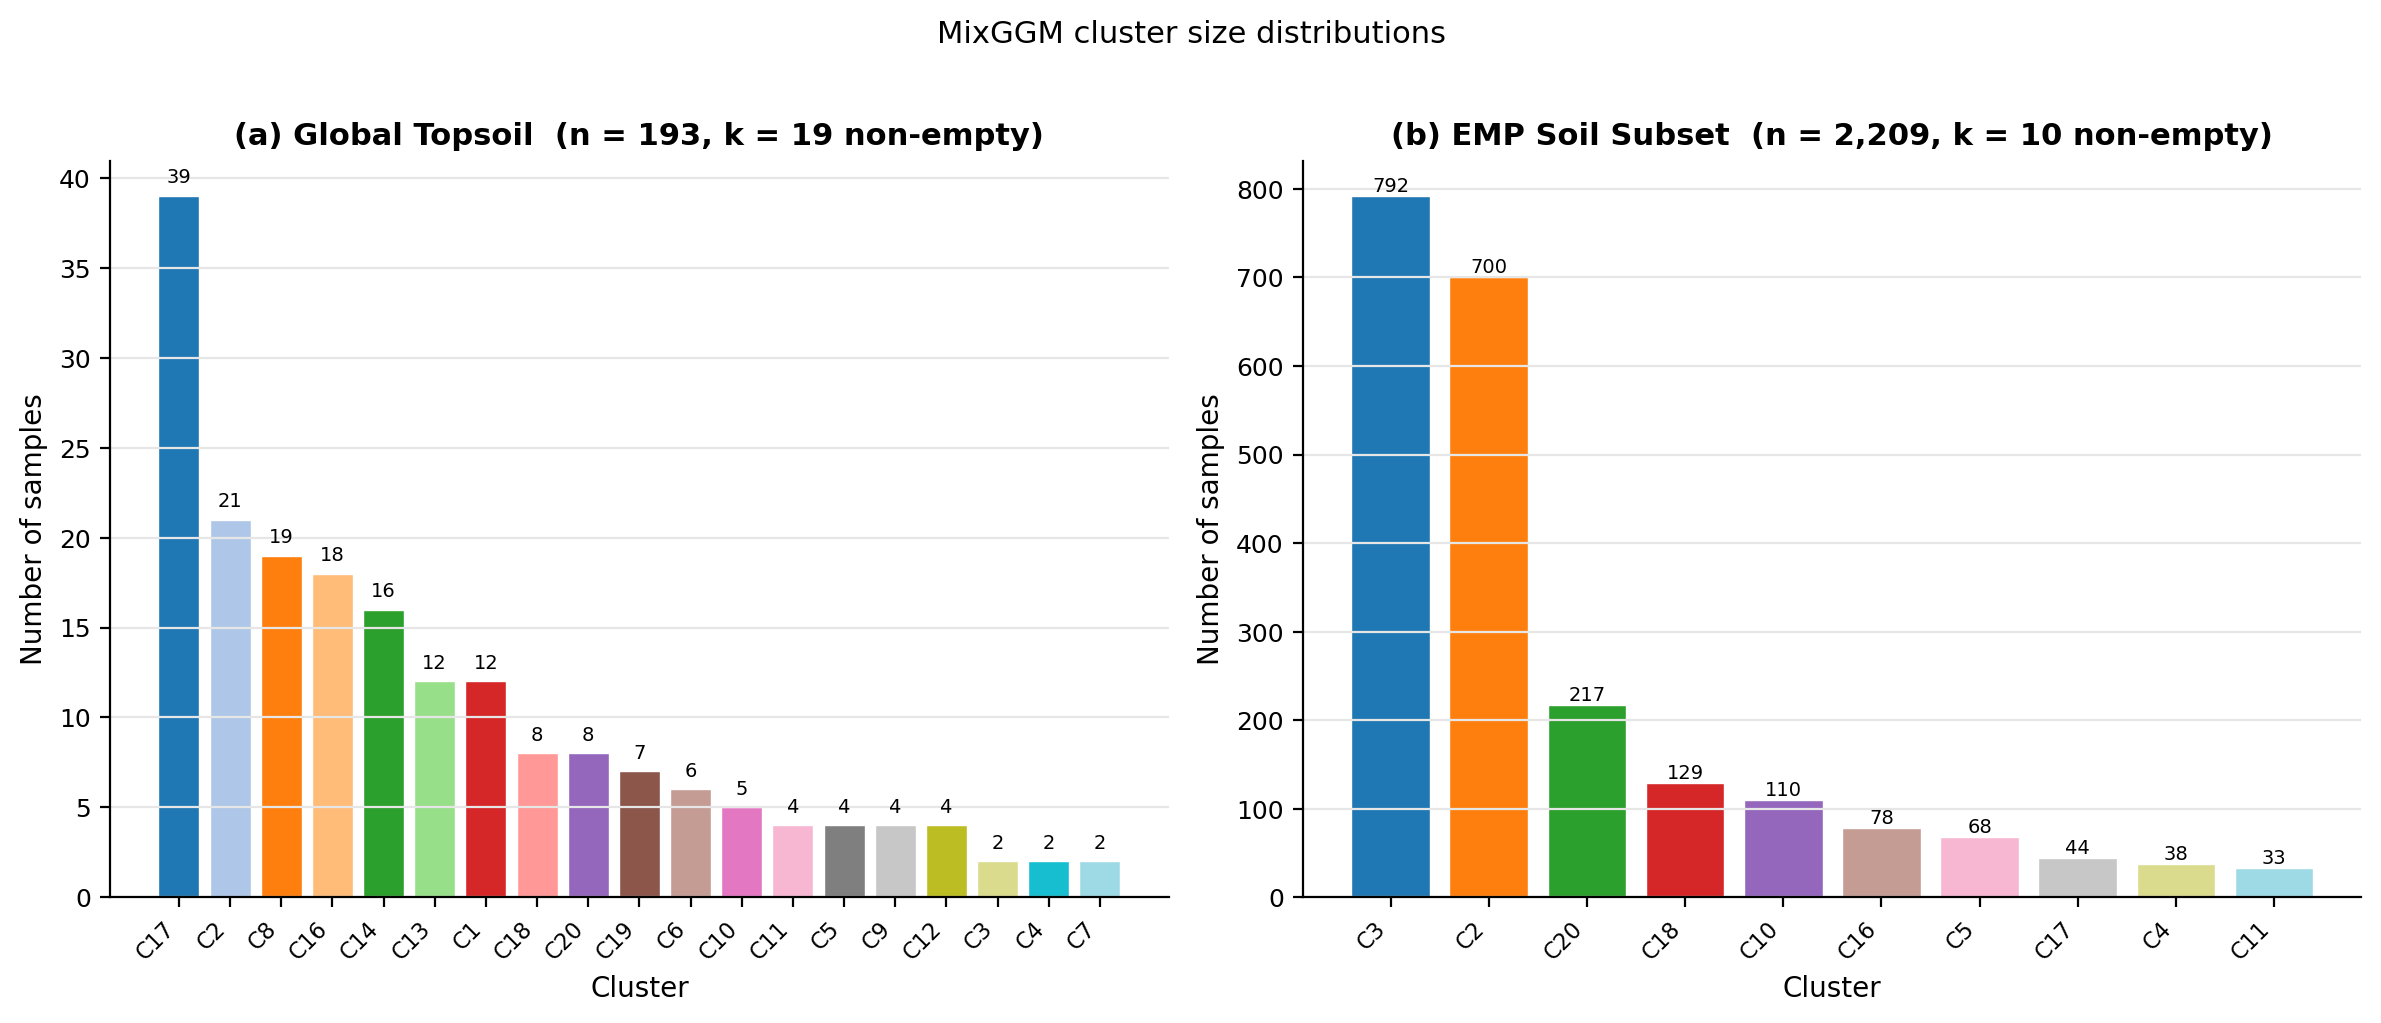
\includegraphics[width=1.05\linewidth]{fig_cluster_sizes.png}
    \caption[MixGGM cluster size distributions]{
    MixGGM cluster size distributions for (a) the global topsoil dataset
    ($n\,=\,193$; $k\,=\,19$ non-empty clusters) and (b) the EMP soil subset
    ($n\,=\,2{,}209$; $k\,=\,10$ non-empty clusters). Bar heights indicate the number
    of samples assigned to each cluster. Clusters are labeled C1--C20 (global topsoil)
    and C2--C20 (EMP), with empty clusters absent.
  }
  \label{fig:7}
\end{figure}

%------------------------------------------------------------
\section{Cluster Characterization by Metadata}
\label{res:char}
%------------------------------------------------------------

The association between cluster assignments and sample metadata was evaluated using
chi-squared tests for categorical variables and Kruskal-Wallis tests for continuous variables;
results for all tested variables are provided in Supplementary Table~4. For the global topsoil
dataset, cluster assignment was significantly associated with annotated biome type
($\chi^2$ $p\,=\,6.1\times10^{-28}$, Cram\'{e}r's $V\,=\,0.485$), country of collection
($p\,=\,4.5\times10^{-8}$, Cram\'{e}r's $V\,=\,0.503$), and latitude (Kruskal-Wallis
$p\,=\,2.9\times10^{-9}$, $\varepsilon^2\,=\,0.339$), but not longitude ($p\,=\,0.050$). The
biome composition of each cluster is shown in Figure~\ref{fig:8}. No cluster was exclusively
composed of a single biome; however, several clusters showed strong biome enrichment.
Cluster~17, the largest cluster ($n\,=\,39$), was dominated by tropical forest samples,
18 of 39 from moist tropical forests and four from tropical montane forests, spanning sites in
Colombia, Papua New Guinea, and Australia. Cluster~1 ($n\,=\,12$) was enriched for savanna
and dry tropical forest samples (7 savanna, 3 dry tropical forest). Cluster~16 ($n\,=\,18$) was
enriched for boreal and coniferous environments (9 boreal forest, 3 temperate coniferous,
3 southern temperate). Cluster~8 ($n\,=\,19$) was predominantly composed of temperate
deciduous forest samples (12 of 19). Cluster~13 ($n\,=\,12$) drew from boreal and southern
temperate biomes in roughly equal proportions (4 boreal, 4 southern temperate, 2 temperate
deciduous, 1 temperate coniferous, 1 arctic tundra), and was the only cluster to contain the
single arctic tundra sample.

For the EMP soil subset, cluster membership showed stronger associations with
environmental classification variables at all hierarchical levels. EMPO level-3 habitat
classification was most strongly associated with cluster assignment
($\chi^2$ $p\,\approx\,0$, Cram\'{e}r's $V\,=\,0.819$), followed by \texttt{env\_material}
(Cram\'{e}r's $V\,=\,0.743$) and \texttt{envo\_biome\_2} (Cram\'{e}r's $V\,=\,0.597$).
Among continuous variables, pH was most strongly structured
(Kruskal-Wallis $\varepsilon^2\,=\,0.741$, $p\,\approx\,0$), followed by salinity
($\varepsilon^2\,=\,0.777$, $p\,\approx\,0$) and elevation ($\varepsilon^2\,=\,0.614$,
$p\,\approx\,0$). The 10 populated clusters separated by habitat type: Clusters~20 ($n\,=\,217$)
and~11 ($n\,=\,33$) comprised entirely of marine saline sediment; Clusters~2 ($n\,=\,700$) and
16 ($n\,=\,78$) were dominated by anthropogenic terrestrial soil; Cluster~17 ($n\,=\,44$)
comprised exclusively freshwater sediment; and Cluster~18 ($n\,=\,129$) was enriched for
plant rhizosphere samples (73 of 129, with the remainder non-saline soil). The biome
composition of each EMP cluster is shown in Figure~\ref{fig:8}.

%--- Figure 8 placeholder -----------------------------------
\begin{figure}[H]
  \centering
  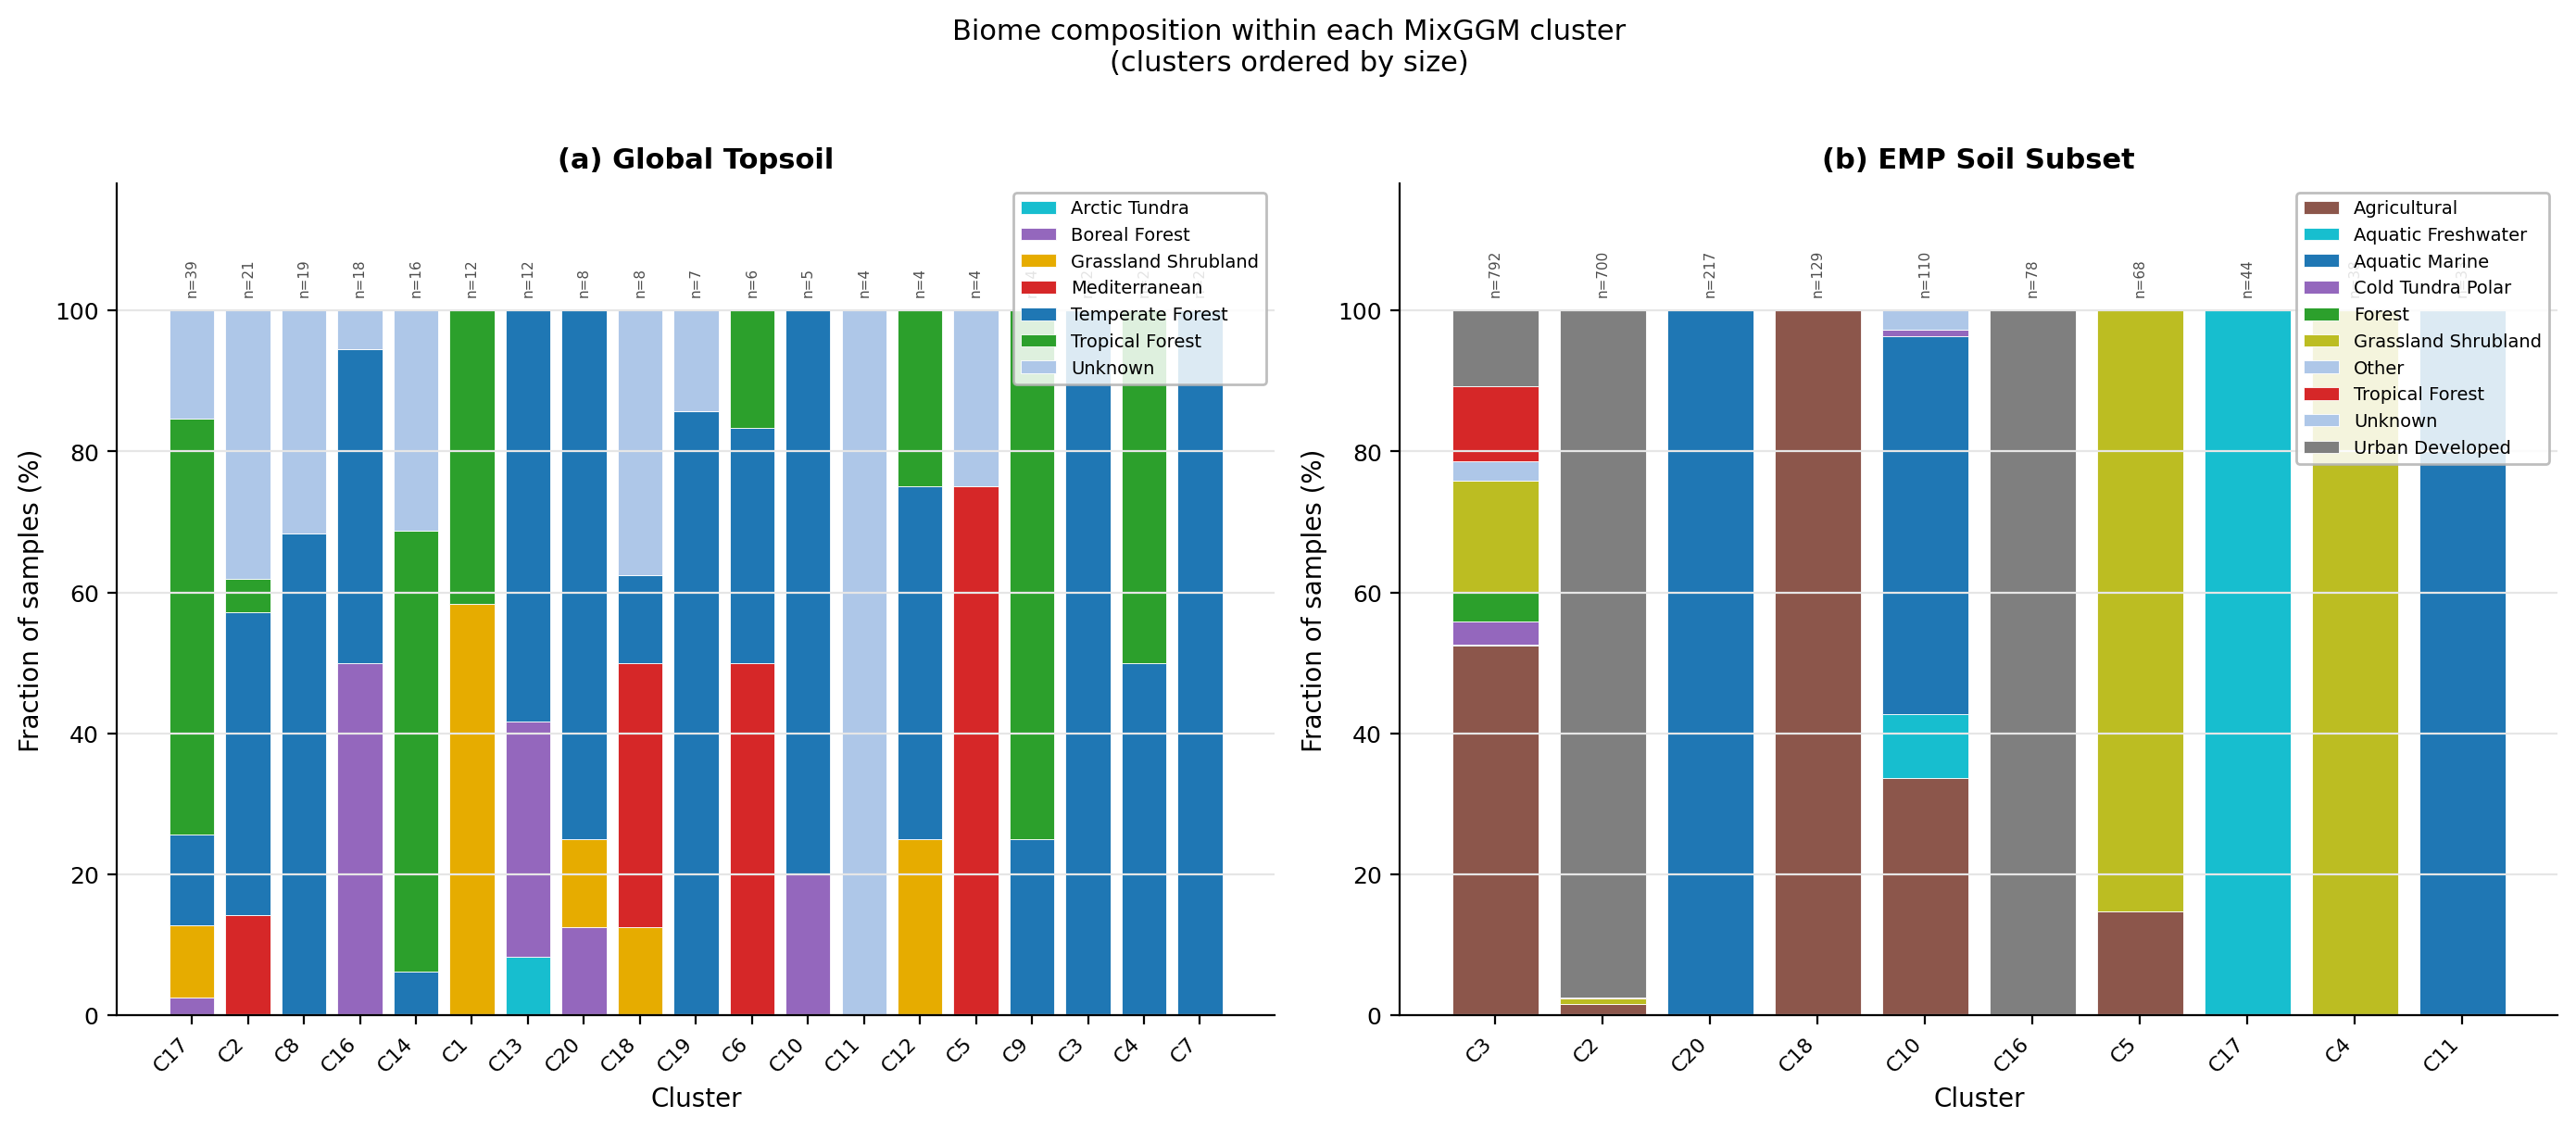
\includegraphics[width=1.05\linewidth]{fig_biome_per_cluster.png}
    \caption[Biome composition within each MixGGM cluster]{
    Biome composition within each MixGGM cluster for (a) the global topsoil dataset
    and (b) the EMP soil subset (clusters ordered by size). The y-axis shows the
    fraction of samples (\%) within each cluster assigned to each biome category. Color
    legend indicates biome type. Global topsoil biome categories include Arctic Tundra,
    Boreal Forest, Grassland/Shrubland, Mediterranean, Temperate Forest, Tropical
    Forest, and Unknown. EMP biome categories include Agricultural, Aquatic Freshwater,
    Aquatic Marine, Cold Tundra Polar, Forest, Grassland/Shrubland, Other, Tropical
    Forest, Unknown, and Urban/Developed.
  }
  \label{fig:8}
\end{figure}

%------------------------------------------------------------
\section{Alpha Diversity Analysis}
\label{res:alpha}
%------------------------------------------------------------

Observed richness, Chao1 richness (Chao 1984)\cite{chao1984}, and Shannon entropy
(Shannon 1948)\cite{shannon1948} were computed per sample and compared across cluster
assignments for both datasets (Figure~\ref{fig:9}).

For the global topsoil dataset, alpha diversity varied across the 19 populated clusters.
Among clusters with four or more samples, mean observed genus richness ranged from 244.2
(Cluster~9) to 708.8 (Cluster~20), and Shannon entropy ranged from 5.18 (Cluster~9) to 6.23
(Cluster~20). Cluster~9 showed the lowest values across all three diversity metrics. Chao1
richness estimates tracked observed richness closely in all clusters. The three clusters with only
two samples (Clusters~3, 4, and~7) showed the most variable diversity estimates. Per-sample
alpha diversity values and cluster-level summary statistics are provided in Supplementary
Table~4.

For the EMP soil subset, alpha diversity varied far more broadly across the 10 populated
clusters, along with the habitat diversity of that dataset. Mean observed genus richness ranged
from 289.4 (Cluster~10) to 5,402.1 (Cluster~5), and Shannon entropy ranged from 2.67
(Cluster~10) to 7.40 (Cluster~18). Cluster~16 showed the lowest within-cluster Shannon
standard deviation of all clusters.

%--- Figure 9 placeholder -----------------------------------
\begin{figure}[H]
  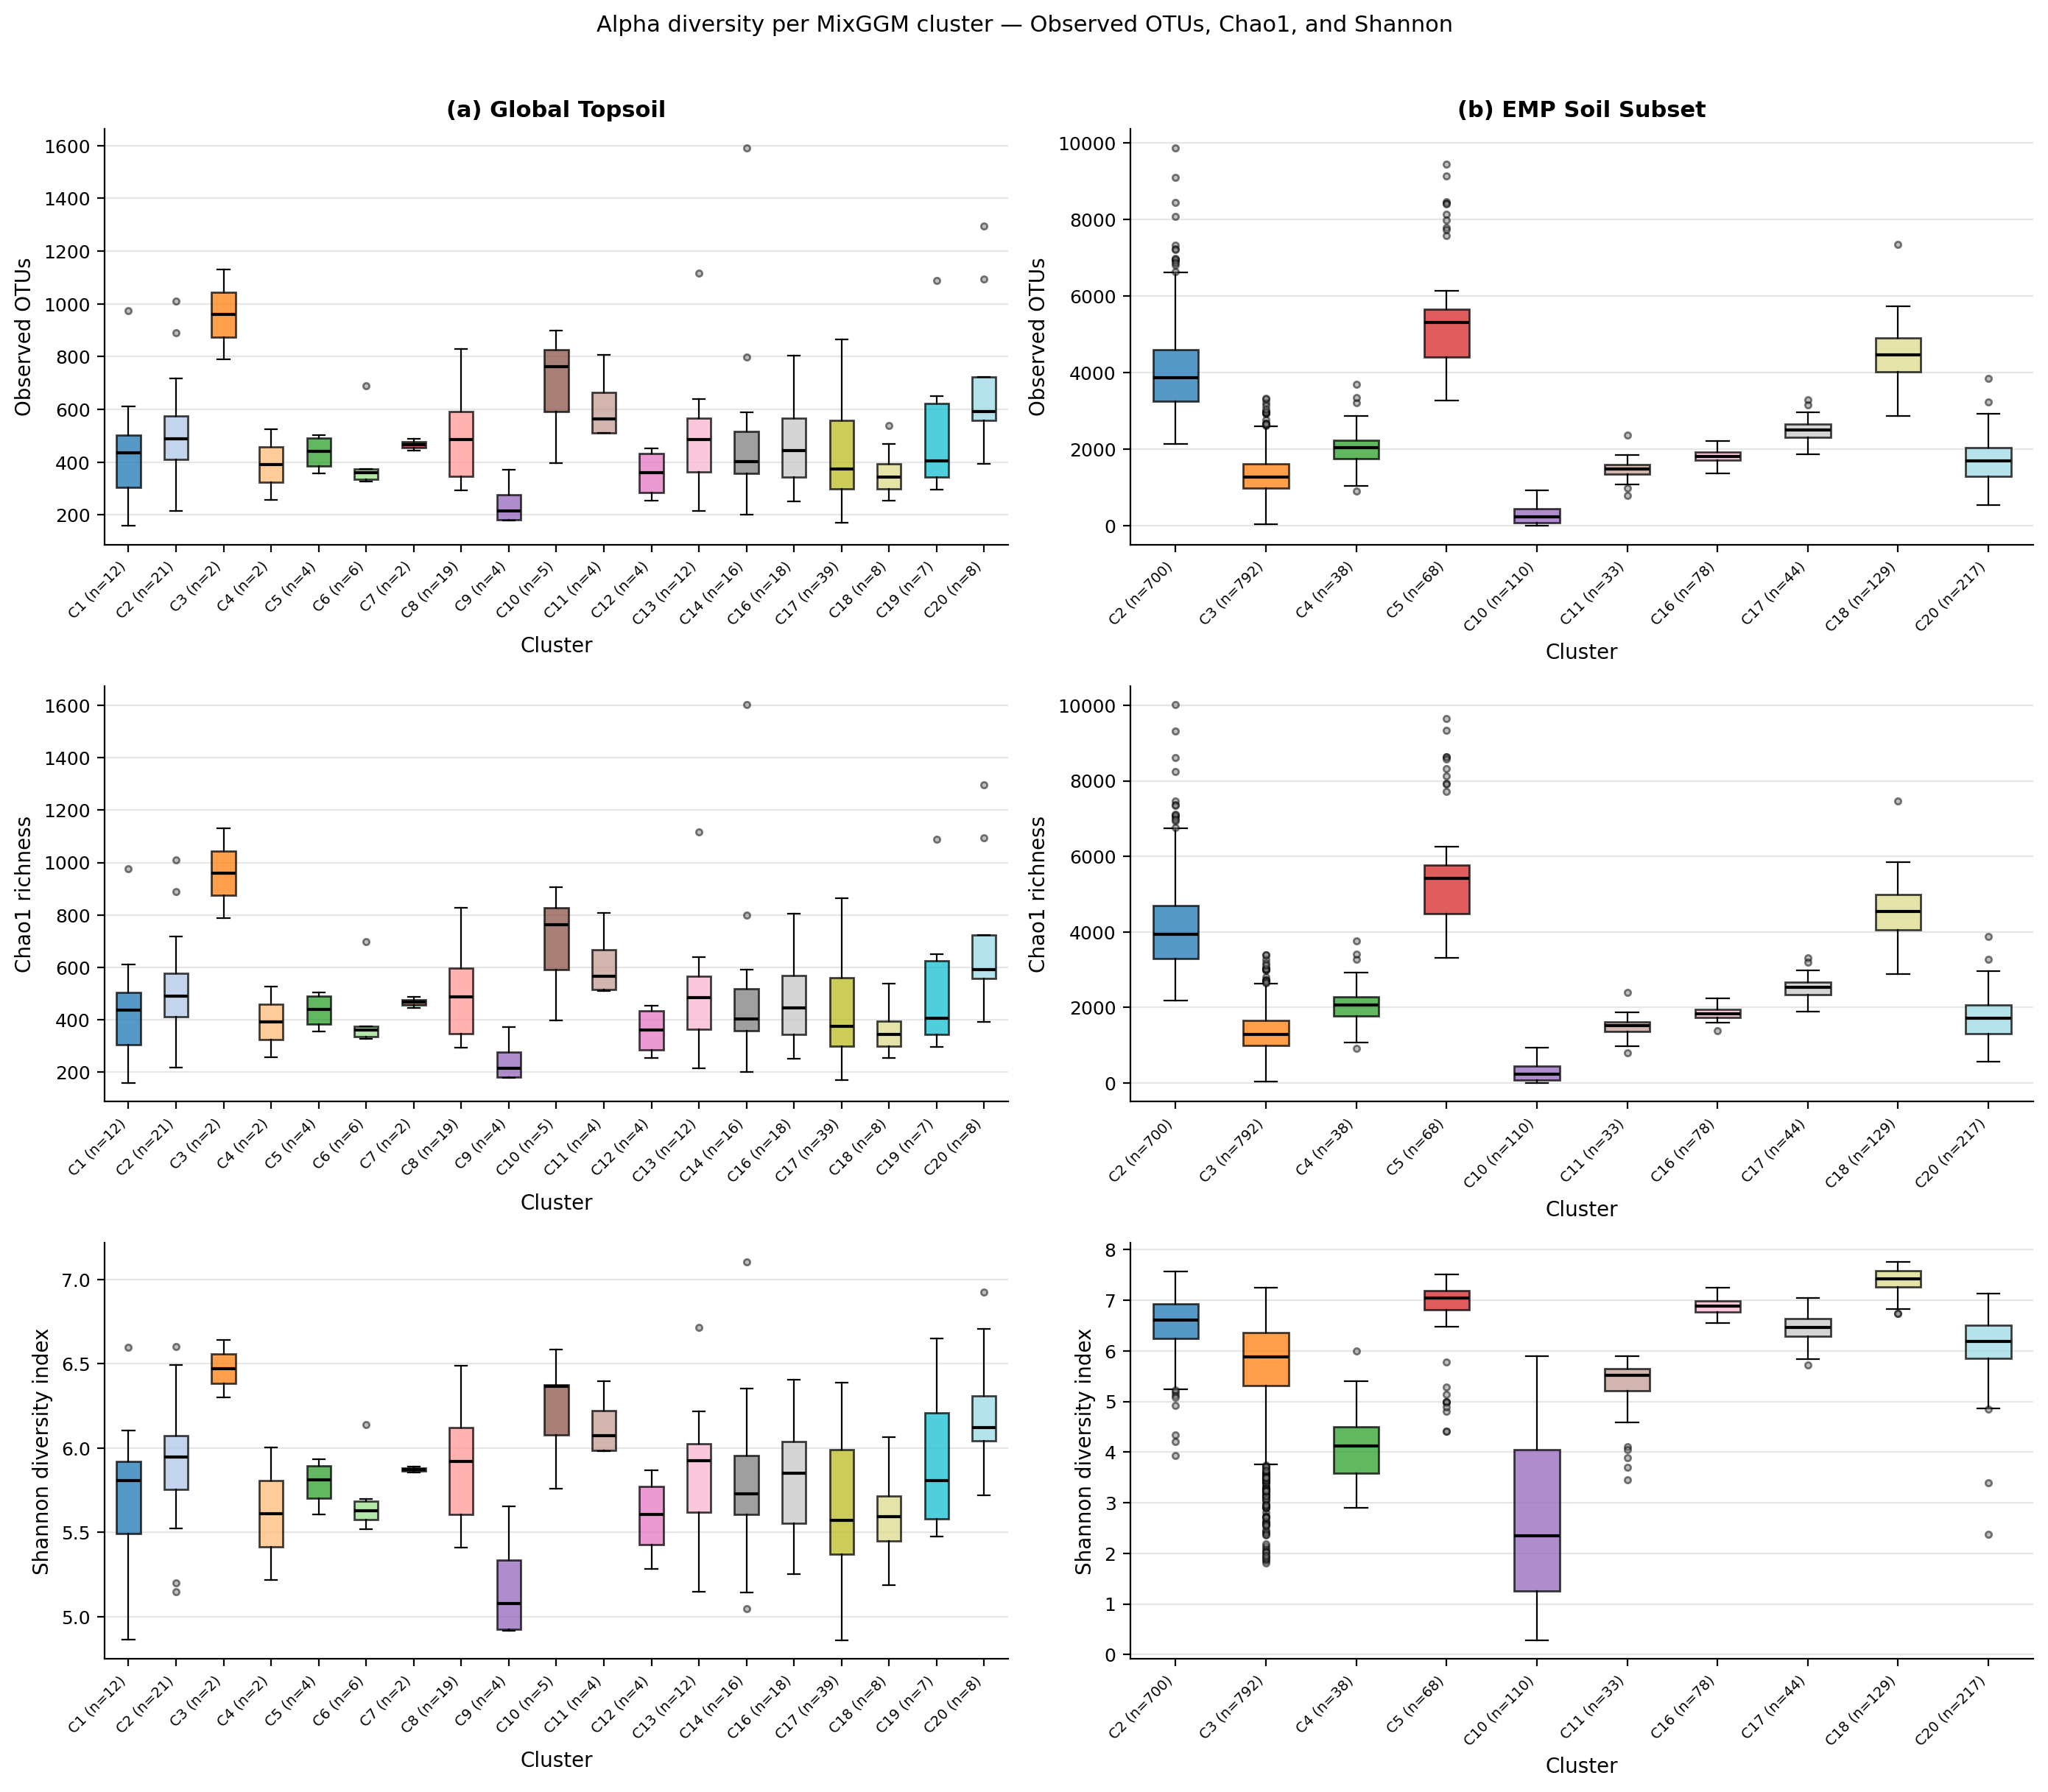
\includegraphics[width=1.05\linewidth] {fig_alpha_diversity_by_cluster.png}
    \caption[Alpha diversity per MixGGM cluster]{
    Alpha diversity per MixGGM cluster for (a) the global topsoil dataset and (b) the
    EMP soil subset. Three metrics are shown (rows): observed OTUs, Chao1 richness, and
    Shannon diversity index. Box plots show median, interquartile range, and outliers.
    Cluster labels on the x-axis include sample size in parentheses. Asterisks ($*$)
    indicate outlier samples.
  }
  \label{fig:9}
\end{figure}

%------------------------------------------------------------
\section{Ordination}
\label{res:ordination}
%------------------------------------------------------------

PCA, PCoA, and t-SNE were applied to both CLR-transformed feature matrices. PCA
biplots and variance scree plots for both datasets are shown in Figure~\ref{fig:10};
t-SNE projections are shown in Figure~\ref{fig:11}. Ordination scores for all methods,
with cluster labels and biome codes, are provided in Supplementary Table~5. PCoA on
CLR-transformed data is mathematically equivalent to CLR-PCA.

For the global topsoil dataset, 20 principal components (PCs) were retained; PC1
explained 20.0\% of total variance and PC2 explained 6.3\%, with the first three components
together accounting for 32.1\% and the first ten components explaining 50.7\%. In the PCA
biplot, MixGGM clusters showed partial separation primarily along PC1; boreal samples
occupied predominantly positive PC1 scores.

For the EMP soil subset, 20 PCs were also retained; PC1 accounted for 41.4\% of
variance, PC2 for 10.1\%, and the first three components together for 56.8\%. The first ten
components explained 70.4\% of total variance. In the PCA biplot, MixGGM clusters showed
strong separation along the first two PCs, with marine and aquatic clusters clearly
distinguished from terrestrial clusters.

%--- Figure 10 placeholder -----------------------------------
\begin{figure}[H]
  \centering
  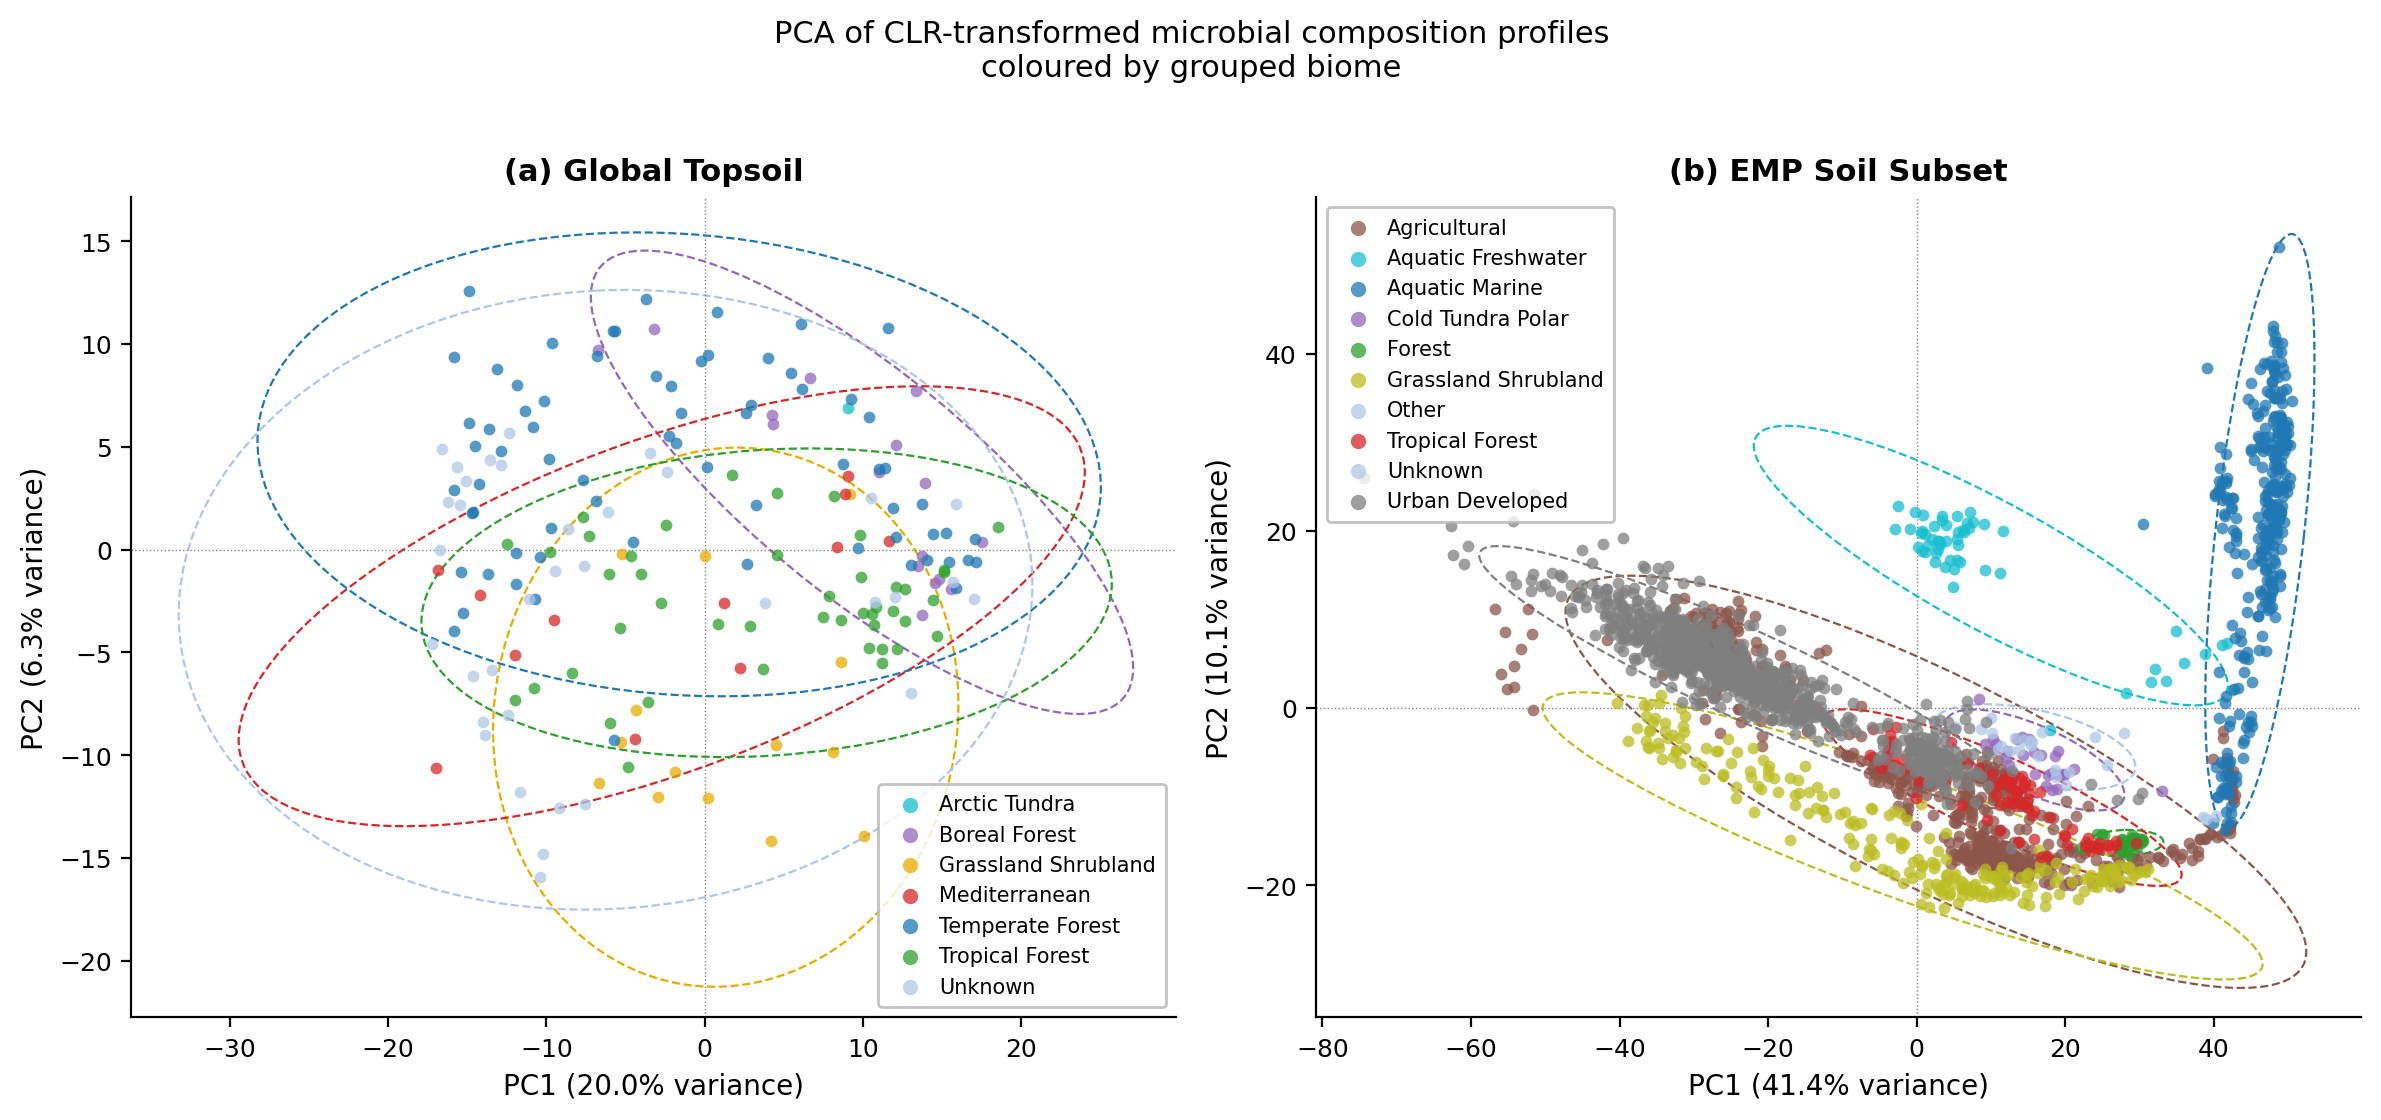
\includegraphics[width=1\linewidth] {fig_pca_both_datasets.png}
  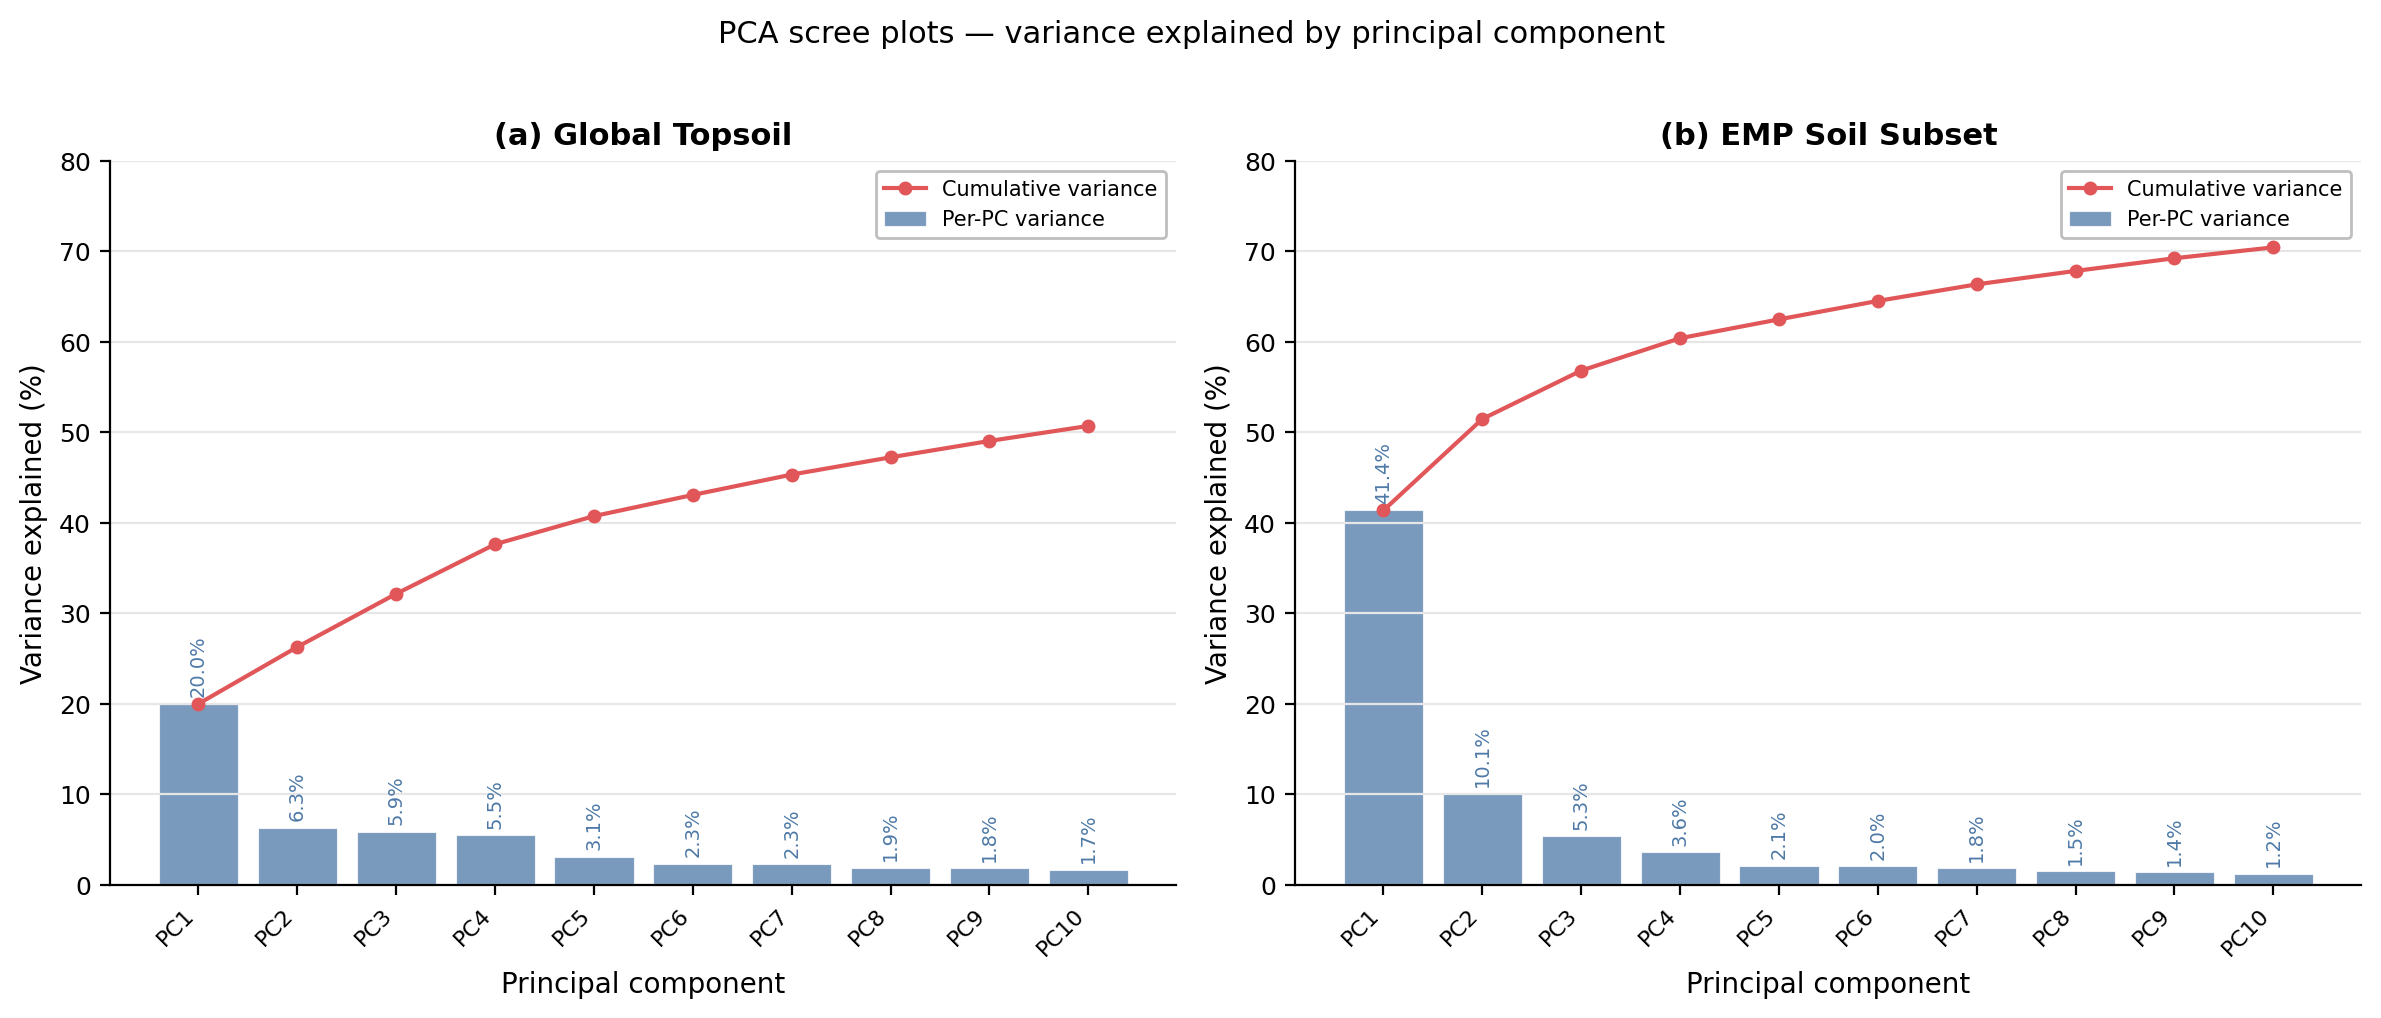
\includegraphics[width=1\linewidth] {fig_pca_scree.png}
    \caption[PCA of CLR-transformed microbial composition profiles]{
    PCA of CLR-transformed microbial composition profiles, coloured by grouped biome,
    for (a) the global topsoil dataset and (b) the EMP soil subset. Dashed ellipses
    indicate 95\% concentration ellipses per biome group. Below: PCA scree plots showing
    per-PC variance (bars) and cumulative variance explained (red line) for the first
    ten components.
  }
  \label{fig:10}
\end{figure}

%--- Figure 11 placeholder -----------------------------------
\begin{figure}[H]
  \centering
  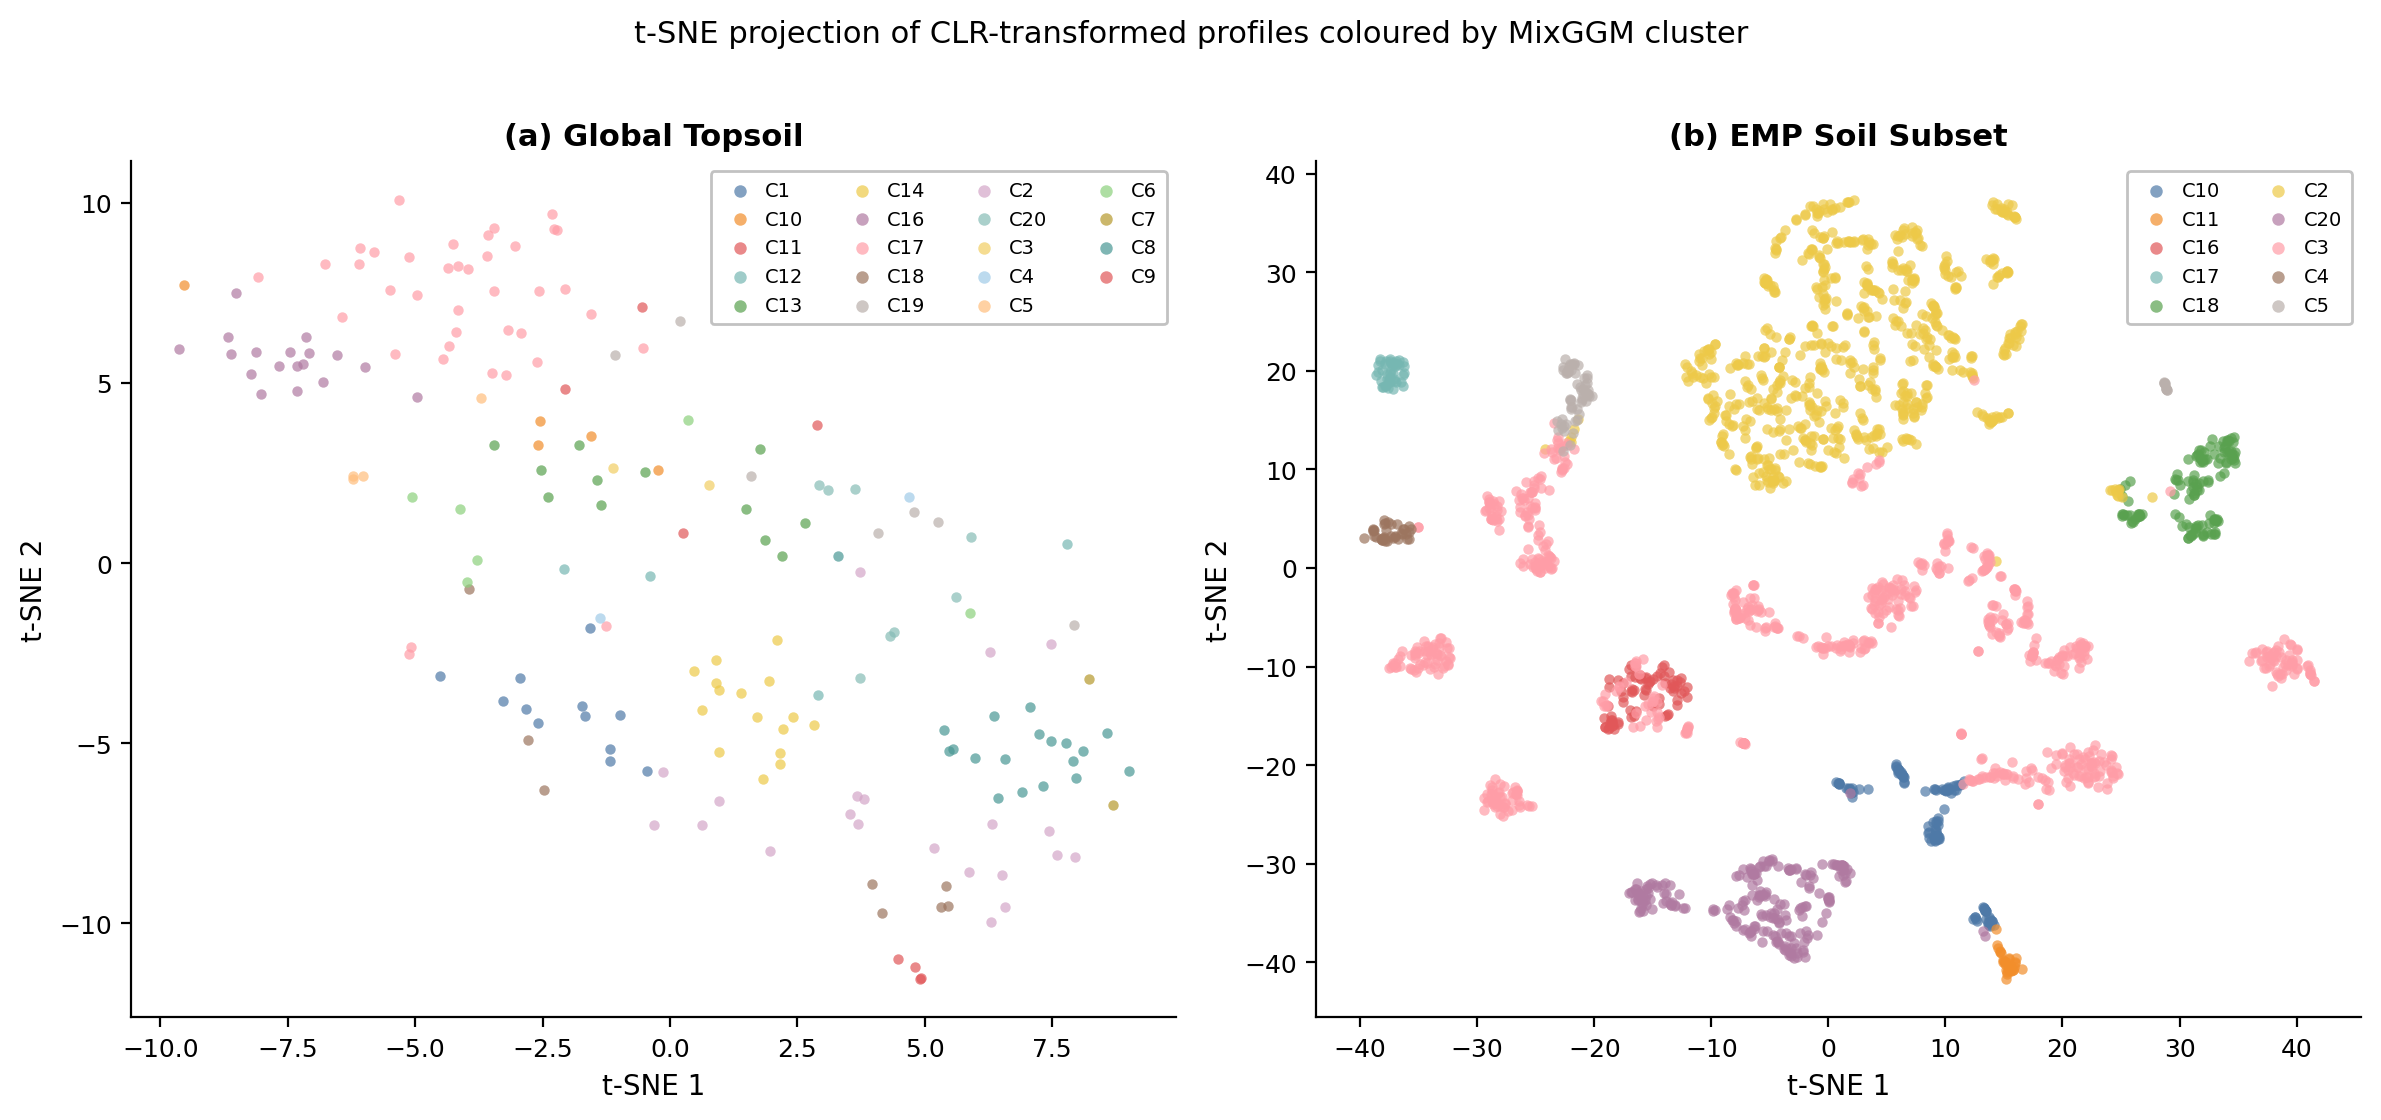
\includegraphics[width=1\linewidth] {fig_tsne_both_datasets.png}
    \caption[t-SNE projection of CLR-transformed profiles]{
    t-SNE projection of CLR-transformed profiles coloured by MixGGM cluster assignment
    for (a) the global topsoil dataset and (b) the EMP soil subset. Each point
    represents one sample. Cluster labels correspond to those in Figure~\ref{fig:7}.
  }
  \label{fig:11}
\end{figure}

%------------------------------------------------------------
\section{Random Forest Biome Classification}
\label{res:rf}
%------------------------------------------------------------

Random Forest classifiers were trained to predict biome of origin from CLR-transformed
microbial composition. Four classifiers were trained in total, one for each combination of
dataset (global topsoil, EMP soil subset) and label scheme (original, grouped biomes).
Test-set performance metrics and full feature importance rankings are provided in
Supplementary Table~6.

For the global topsoil dataset, eight original biome classes were retained for classifier
training; consolidation into grouped labels reduced this to six classes after exclusion of Arctic
Tundra ($n\,=\,1$). Under original biome labels, the Random Forest achieved 43.75\%
test-set accuracy (Cohen's $\kappa\,=\,0.327$). Grouping biomes into six broader categories
improved accuracy to 61.82\% ($\kappa\,=\,0.441$), with Grassland/Shrubland and
Mediterranean categories too small to appear in the 30\% test split and not contributing to
the grouped accuracy estimate. Within the original label model, the moist tropical forest class
showed the highest recall of the larger classes (63.6\%), while the southern temperate forest
class showed the lowest recall (14.3\%), with misclassification distributed across multiple
other temperate categories. Under grouped labels, the Tropical Forest group showed the best
recall of the four evaluable classes (75.0\%), followed by Temperate Forest (55.9\%). The most
predictive lineages by permutation importance (MDA) under original biome labels were
\textit{Ellin516} (MDA\,=\,7.97), \textit{Tundrisphaera} (MDA\,=\,7.80), and
\textit{Pedomicrobium} (MDA\,=\,7.73). Under grouped labels, \textit{Ellin516}
(MDA\,=\,7.47), \textit{Anaeromyxobacter} (MDA\,=\,7.31), and \textit{Bacillus}
(MDA\,=\,6.58) ranked highest. Top lineage importances for both topsoil models are shown
in Figure~\ref{fig:12}.

For the EMP soil subset, the same architecture was applied to 11 original and 9 grouped
biome classes. Classification performance was higher than in the global topsoil dataset:
test-set accuracy was 97.11\% under original biome labels ($\kappa\,=\,0.961$) and 98.17\%
under grouped labels ($\kappa\,=\,0.975$). The confusion matrix for original biome labels
showed near-perfect diagonal results for most classes: marine (92 of 92), montane grassland
(68 of 68), urban (252 of 252), small river (13 of 13), and tropical moist broadleaf forest
(22 of 22) were all classified with perfect test-set recall. The cropland class showed the most
misclassification (12 of 183 errors, primarily predicted as rangeland), and tundra samples
showed the second-highest error rate (3 of 9 test samples predicted as freshwater). The top
predictive lineages under original biome labels were \textit{Sphingomonas} (MDA\,=\,10.76),
\textit{Paenibacillus} (MDA\,=\,10.67), and \textit{Candidatus} Udaeobacter
(MDA\,=\,9.39). Under grouped labels, \textit{Paenibacillus} (MDA\,=\,10.19),
ADurb.Bin063-1 (MDA\,=\,9.54), and \textit{Planococcaceae} (MDA\,=\,9.46) ranked
highest. Top lineage importances for both EMP models are shown in Figure~\ref{fig:12}.

%--- Figure 12 placeholder ----------------------------------
\begin{figure}[H]
  \centering
  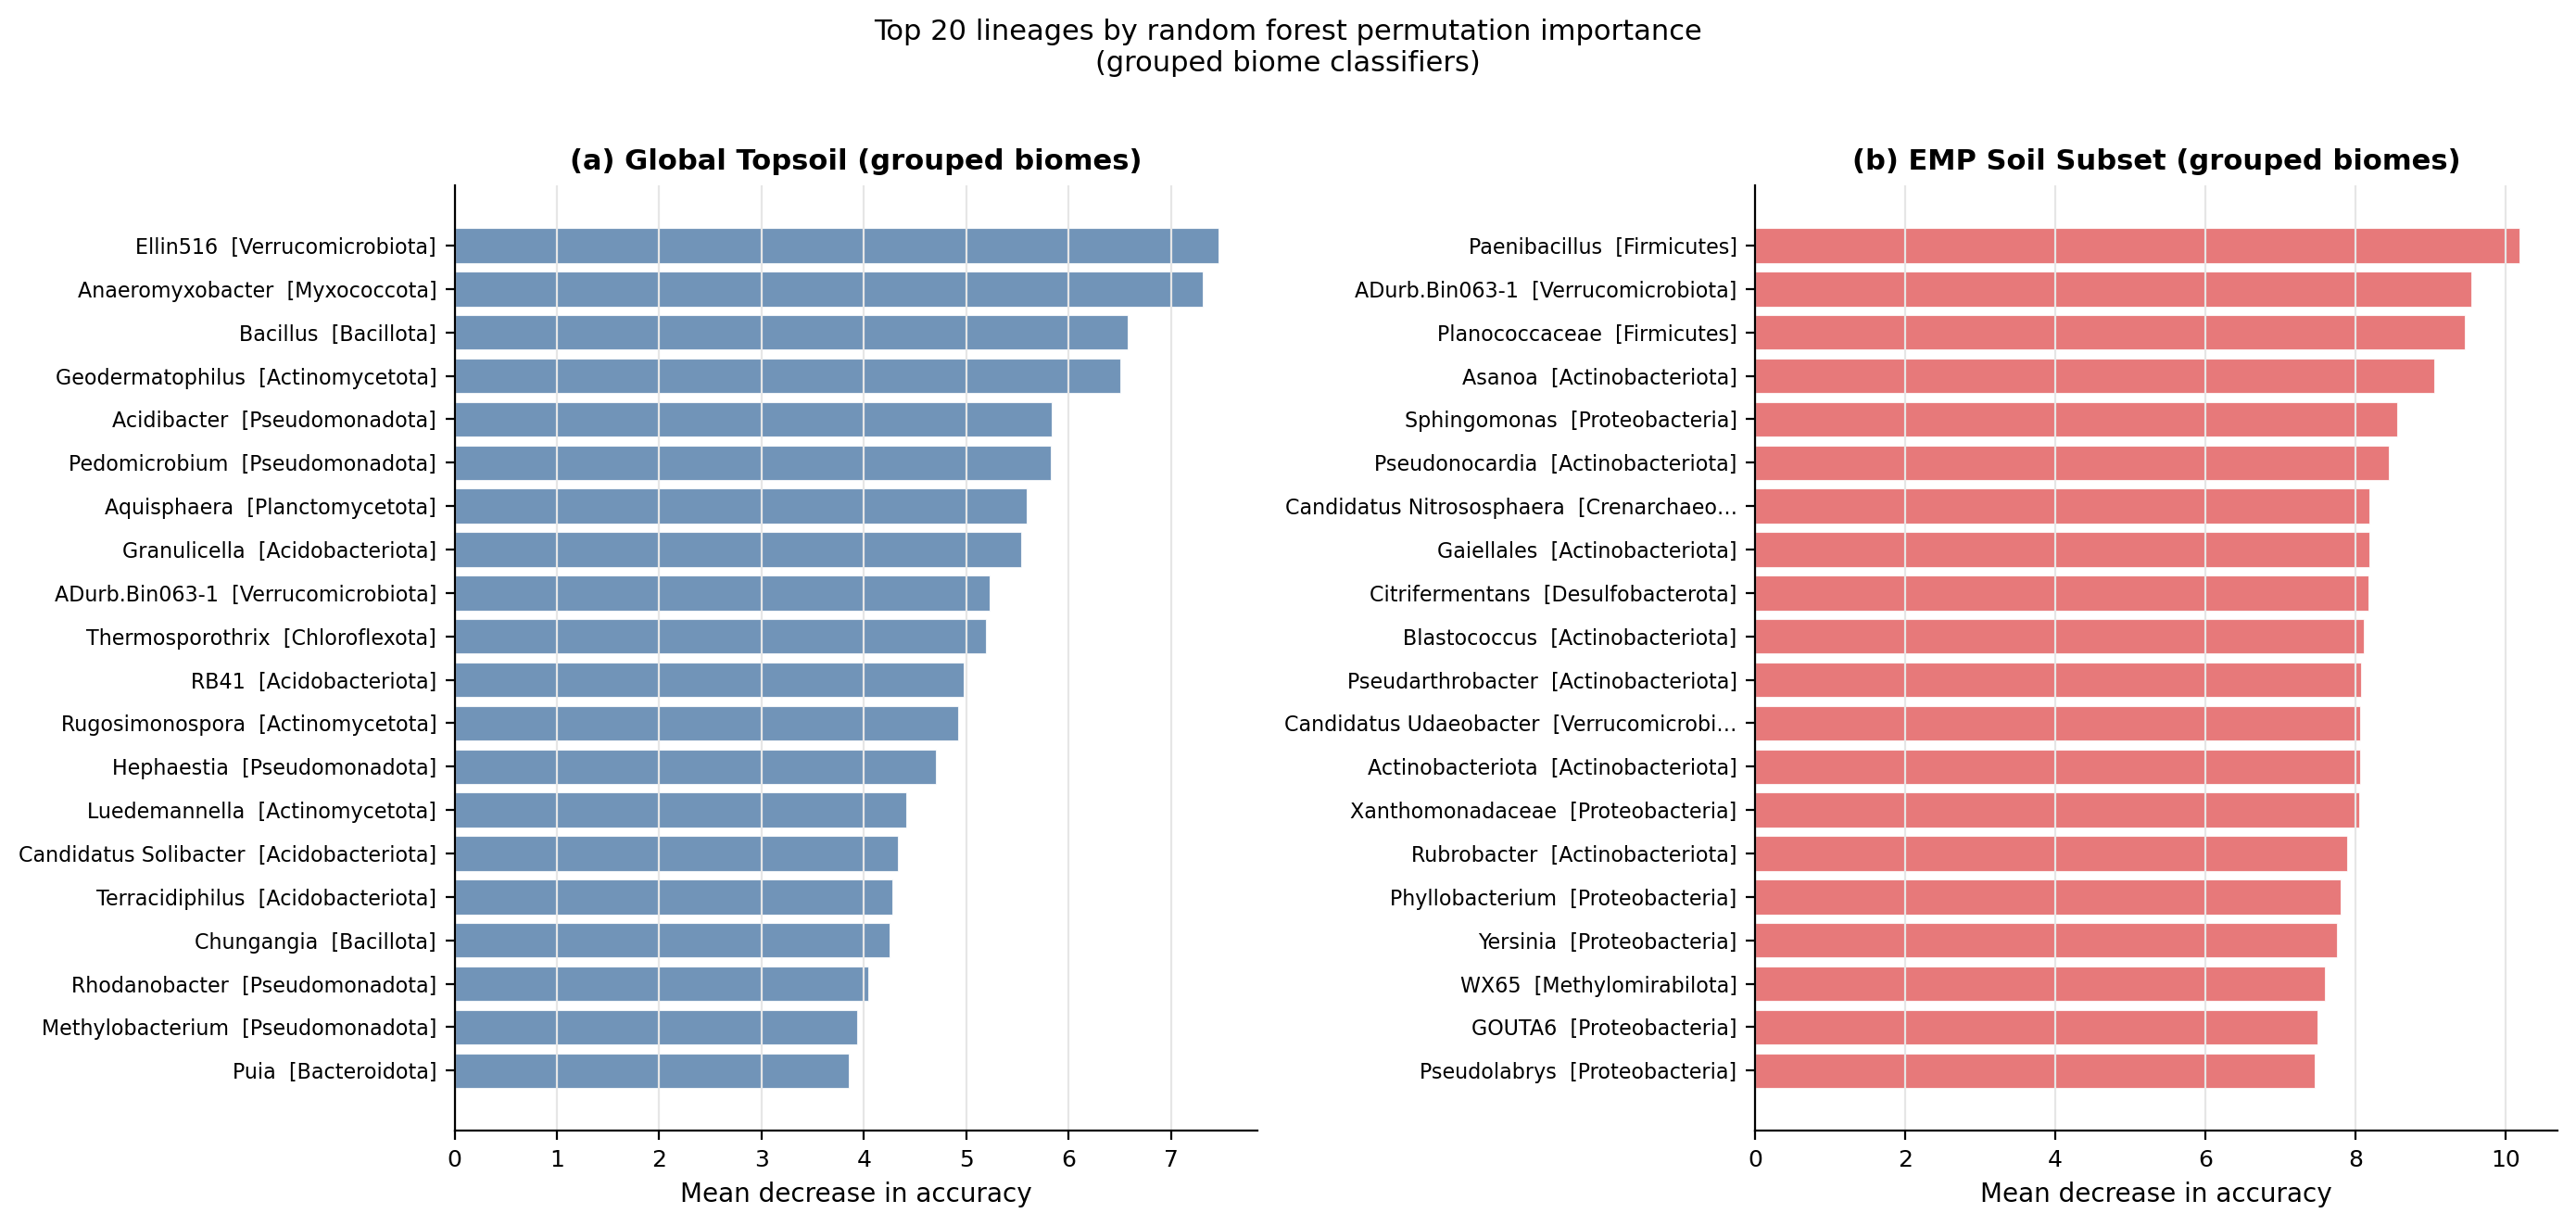
\includegraphics[width=1.05\linewidth] {fig_rf_feature_importance.png}
    \caption[Top 20 lineages by random forest permutation importance]{
    Top 20 lineages by random forest permutation importance (MeanDecreaseAccuracy)
    under grouped biome classifiers for (a) the global topsoil dataset and (b) the EMP
    soil subset. Bars indicate MDA values; lineage names include phylum-level
    classification in brackets. Bacterial lineage names are italicized where they refer
    to named genera.
  }
  \label{fig:12}
\end{figure}

%============================================================
\chapter{Discussion}
%============================================================

[Discussion text to be inserted here.]

%============================================================
\chapter{Conclusion}
%============================================================

[Conclusion text to be inserted here.]

%============================================================
% BIBLIOGRAPHY
%============================================================
\newpage
\addcontentsline{toc}{chapter}{References}

\begin{thebibliography}{99}

\bibitem{aitchison1986}
Aitchison J. 1986.
\textit{The Statistical Analysis of Compositional Data}.
Chapman and Hall, London.

\bibitem{amir2017}
Amir A, McDonald D, Navas-Molina JA, Kopylova E, Morton JT, Xu ZZ, Kightley EP,
Thompson LR, Hyde ER, Gonzalez A, Knight R. 2017.
Deblur rapidly resolves single-nucleotide community sequence patterns.
\textit{mSystems} 2:e00191-16.

\bibitem{bahram2018}
Bahram M, Hildebrand F, Forslund SK, Anderson JL, Soudzilovskaia NA, Bodegom PM,
Bengtsson-Palme J, Anslan S, Coelho LP, Harend H, et al. 2018.
Structure and function of the global topsoil microbiome.
\textit{Nature} 560:233--237.

\bibitem{breiman2001}
Breiman L. 2001.
Random forests.
\textit{Machine Learning} 45:5--32.

\bibitem{callahan2016}
Callahan BJ, McMurdie PJ, Rosen MJ, Han AW, Johnson AJA, Holmes SP. 2016.
DADA2: High-resolution sample inference from Illumina amplicon data.
\textit{Nature Methods} 13:581--583.

\bibitem{chao1984}
Chao A. 1984.
Nonparametric estimation of the number of classes in a population.
\textit{Scandinavian Journal of Statistics} 11:265--270.

\bibitem{dixon2003}
Dixon P. 2003.
VEGAN, a package of R functions for community ecology.
\textit{Journal of Vegetation Science} 14:927--930.

\bibitem{fierer2006}
Fierer N, Jackson RB. 2006.
The diversity and biogeography of soil bacterial communities.
\textit{Proceedings of the National Academy of Sciences} 103:626--631.

\bibitem{gower1966}
Gower JC. 1966.
Some distance properties of latent root and vector methods used in multivariate analysis.
\textit{Biometrika} 53:325--338.

\bibitem{maaten2008}
van der Maaten L, Hinton G. 2008.
Visualizing data using t-SNE.
\textit{Journal of Machine Learning Research} 9:2579--2605.

\bibitem{mcmurdie2013}
McMurdie PJ, Holmes S. 2013.
phyloseq: An R package for reproducible interactive analysis and graphics of
microbiome census data.
\textit{PLOS ONE} 8:e61217.

\bibitem{pearson1901}
Pearson K. 1901.
On lines and planes of closest fit to systems of points in space.
\textit{Philosophical Magazine} 2:559--572.

\bibitem{quast2013}
Quast C, Pruesse E, Yilmaz P, Gerken J, Schweer T, Yarza P, Peplies J,
Gl\"{o}ckner FO. 2013.
The SILVA ribosomal RNA gene database project: improved data processing and
web-based tools.
\textit{Nucleic Acids Research} 41:D590--D596.

\bibitem{shannon1948}
Shannon CE. 1948.
A mathematical theory of communication.
\textit{Bell System Technical Journal} 27:379--423.

\bibitem{thompson2017}
Thompson LR, Sanders JG, McDonald D, Amir A, Ladau J, Locey KJ, Prill RJ,
Tripathi A, Gibbons SM, Ackermann G, et al. 2017.
A communal catalogue reveals Earth's multiscale microbial diversity.
\textit{Nature} 551:457--463.

\bibitem{yooseph2022}
Yooseph S. 2022.
[Full citation for MixGGM paper to be confirmed and inserted here.]

\end{thebibliography}


%============================================================
%============================================================
\appendix
\chapter{Supplementary Tables}
\label{app:supp}
%============================================================

The following supplementary tables provide complete per-sample and per-cluster statistics
supporting the results reported in the main text. Tables 4a and 4d (per-sample data) and
Table 5a (ordination scores) are provided as separate CSV files due to their size;
all other supplementary tables are reproduced in full below.

\newpage

%------------------------------------------------------------
\section*{Supplementary Table 1: DADA2 Read Tracking --- Global Topsoil Dataset}
\addcontentsline{toc}{section}{Supplementary Table 1}
\label{supp:tab1}
%------------------------------------------------------------

Per-sample read counts at each DADA2 pipeline stage for all 234 downloaded samples
from EBI accession PRJEB19856. \textbf{Input} = raw reads;
\textbf{Filt} = reads after \texttt{filterAndTrim()};
\textbf{\%Filt} = \% retained after filtering;
\textbf{Denois} = reads after \texttt{dada()} denoising;
\textbf{Merged} = reads after \texttt{mergePairs()};
\textbf{\%Mrgd} = \% of input retained after merging;
\textbf{Non-chim} = reads after \texttt{removeBimeraDenovo()};
\textbf{\%NC} = \% of input retained as non-chimeric;
\textbf{\%F$\to$M} = \% of filtered reads that merged;
\textbf{\%M$\to$NC} = \% of merged reads that are non-chimeric;
\textbf{ASVs} = unique ASVs detected.

\begingroup\fontsize{7}{9}\selectfont
\begin{longtable}{@{}p{3.2cm}rrrrrrrrrrr@{}}
\caption[DADA2 read tracking --- Global Topsoil]{DADA2 read tracking --- Global Topsoil Dataset (234 samples).}
\label{tab:supp1} \\
\toprule
\textbf{Sample ID} & \textbf{Input} & \textbf{Filt} & \textbf{\%Filt} &
\textbf{Denois} & \textbf{Merged} & \textbf{\%Mrgd} &
\textbf{Non-chim} & \textbf{\%NC} & \textbf{\%F$\to$M} &
\textbf{\%M$\to$NC} & \textbf{ASVs} \\
\midrule
\endfirsthead
\multicolumn{12}{l}{\small\itshape(continued from previous page)} \\[2pt]
\toprule
\textbf{Sample ID} & \textbf{Input} & \textbf{Filt} & \textbf{\%Filt} &
\textbf{Denois} & \textbf{Merged} & \textbf{\%Mrgd} &
\textbf{Non-chim} & \textbf{\%NC} & \textbf{\%F$\to$M} &
\textbf{\%M$\to$NC} & \textbf{ASVs} \\
\midrule
\endhead
\midrule
\multicolumn{12}{r}{\small\itshape(continued on next page)} \\
\endfoot
\bottomrule
\endlastfoot
ERR1873185 & 130154 & 99666 & 76.58 & 93730 & 67354 & 51.75 & 45233 & 34.75 & 67.58 & 67.16 & 840 \\
ERR1873186 & 78022 & 60516 & 77.56 & 55656 & 37504 & 48.07 & 27836 & 35.68 & 61.97 & 74.22 & 416 \\
ERR1873188 & 78755 & 59602 & 75.68 & 54279 & 35323 & 44.85 & 28225 & 35.84 & 59.26 & 79.91 & 372 \\
ERR1873189 & 54735 & 35628 & 65.09 & 31201 & 16963 & 30.99 & 14666 & 26.79 & 47.61 & 86.46 & 128 \\
ERR1873190 & 103976 & 77340 & 74.38 & 72444 & 53360 & 51.32 & 37310 & 35.88 & 68.99 & 69.92 & 536 \\
ERR1873191 & 42999 & 30536 & 71.02 & 26963 & 16765 & 38.99 & 12465 & 28.99 & 54.9 & 74.35 & 149 \\
ERR1873192 & 17691 & 13386 & 75.67 & 10810 & 5727 & 32.37 & 5601 & 31.66 & 42.78 & 97.8 & 60 \\
ERR1873193 & 138850 & 102030 & 73.48 & 93882 & 62536 & 45.04 & 50004 & 36.01 & 61.29 & 79.96 & 816 \\
ERR1873194 & 96676 & 63662 & 65.85 & 58211 & 38292 & 39.61 & 30674 & 31.73 & 60.15 & 80.11 & 380 \\
ERR1873195 & 142219 & 112690 & 79.24 & 103414 & 77239 & 54.31 & 53993 & 37.96 & 68.54 & 69.9 & 792 \\
ERR1873196 & 231008 & 174474 & 75.53 & 157484 & 99705 & 43.16 & 69285 & 29.99 & 57.15 & 69.49 & 966 \\
ERR1873197 & 137515 & 110167 & 80.11 & 100212 & 67767 & 49.28 & 50984 & 37.08 & 61.51 & 75.23 & 873 \\
ERR1873198 & 137117 & 102699 & 74.9 & 90789 & 47487 & 34.63 & 39656 & 28.92 & 46.24 & 83.51 & 566 \\
ERR1873199 & 150040 & 116845 & 77.88 & 103964 & 66603 & 44.39 & 51428 & 34.28 & 57.0 & 77.22 & 803 \\
ERR1873201 & 98381 & 74841 & 76.07 & 67933 & 44564 & 45.3 & 34387 & 34.95 & 59.54 & 77.16 & 588 \\
ERR1873202 & 107673 & 83260 & 77.33 & 74130 & 46336 & 43.03 & 38932 & 36.16 & 55.65 & 84.02 & 609 \\
ERR1873203 & 161414 & 126852 & 78.59 & 113654 & 66692 & 41.32 & 55256 & 34.23 & 52.57 & 82.85 & 764 \\
ERR1873204 & 157637 & 115797 & 73.46 & 106637 & 75395 & 47.83 & 53112 & 33.69 & 65.11 & 70.44 & 877 \\
ERR1873205 & 225732 & 170545 & 75.55 & 159935 & 124198 & 55.02 & 69545 & 30.81 & 72.82 & 56.0 & 1387 \\
ERR1873206 & 175412 & 145527 & 82.96 & 137594 & 113225 & 64.55 & 60450 & 34.46 & 77.8 & 53.39 & 1468 \\
ERR1873207 & 118776 & 85203 & 71.73 & 73231 & 44276 & 37.28 & 32828 & 27.64 & 51.97 & 74.14 & 493 \\
ERR1873208 & 162599 & 128916 & 79.28 & 112433 & 72456 & 44.56 & 52756 & 32.45 & 56.2 & 72.81 & 868 \\
ERR1873209 & 227549 & 176601 & 77.61 & 158856 & 99483 & 43.72 & 67833 & 29.81 & 56.33 & 68.19 & 1281 \\
ERR1873210 & 95463 & 66405 & 69.56 & 52913 & 30665 & 32.12 & 21097 & 22.1 & 46.18 & 68.8 & 216 \\
ERR1873211 & 64164 & 50267 & 78.34 & 40783 & 22242 & 34.66 & 18928 & 29.5 & 44.25 & 85.1 & 312 \\
ERR1873212 & 97726 & 76834 & 78.62 & 65332 & 37659 & 38.54 & 30251 & 30.95 & 49.01 & 80.33 & 376 \\
ERR1873213 & 108132 & 82367 & 76.17 & 68539 & 31695 & 29.31 & 29151 & 26.96 & 38.48 & 91.97 & 328 \\
ERR1873214 & 83927 & 60652 & 72.27 & 52099 & 28618 & 34.1 & 24283 & 28.93 & 47.18 & 84.85 & 267 \\
ERR1873215 & 129361 & 96373 & 74.5 & 85526 & 51914 & 40.13 & 43366 & 33.52 & 53.87 & 83.53 & 632 \\
ERR1873216 & 31652 & 23135 & 73.09 & 19380 & 11159 & 35.26 & 9273 & 29.3 & 48.23 & 83.1 & 107 \\
ERR1873217 & 64178 & 49761 & 77.54 & 39503 & 15568 & 24.26 & 14079 & 21.94 & 31.29 & 90.44 & 183 \\
ERR1873218 & 75009 & 57252 & 76.33 & 50413 & 28707 & 38.27 & 22622 & 30.16 & 50.14 & 78.8 & 332 \\
ERR1873219 & 88608 & 68511 & 77.32 & 57850 & 30412 & 34.32 & 24123 & 27.22 & 44.39 & 79.32 & 327 \\
ERR1873220 & 109483 & 86538 & 79.04 & 73999 & 43983 & 40.17 & 34062 & 31.11 & 50.83 & 77.44 & 552 \\
ERR1873221 & 139041 & 94095 & 67.67 & 84410 & 52854 & 38.01 & 43491 & 31.28 & 56.17 & 82.29 & 598 \\
ERR1873222 & 136622 & 102603 & 75.1 & 88410 & 46955 & 34.37 & 40474 & 29.62 & 45.76 & 86.2 & 514 \\
ERR1873223 & 119334 & 86026 & 72.09 & 75909 & 47198 & 39.55 & 37307 & 31.26 & 54.86 & 79.04 & 571 \\
ERR1873224 & 88604 & 69982 & 78.98 & 57369 & 28871 & 32.58 & 24922 & 28.13 & 41.25 & 86.32 & 356 \\
ERR1873225 & 68231 & 53313 & 78.14 & 49070 & 33849 & 49.61 & 23932 & 35.07 & 63.49 & 70.7 & 459 \\
ERR1873226 & 147620 & 115503 & 78.24 & 96183 & 51451 & 34.85 & 45091 & 30.55 & 44.55 & 87.64 & 623 \\
ERR1873227 & 23615 & 18353 & 77.72 & 15449 & 9057 & 38.35 & 7102 & 30.07 & 49.35 & 78.41 & 116 \\
ERR1873228 & 78308 & 57410 & 73.31 & 51887 & 35954 & 45.91 & 25863 & 33.03 & 62.63 & 71.93 & 454 \\
ERR1873229 & 44835 & 31828 & 70.99 & 26155 & 15643 & 34.89 & 13479 & 30.06 & 49.15 & 86.17 & 178 \\
ERR1873230 & 50310 & 34953 & 69.48 & 31047 & 22070 & 43.87 & 16417 & 32.63 & 63.14 & 74.39 & 251 \\
ERR1873231 & 77158 & 60105 & 77.9 & 52856 & 35371 & 45.84 & 27807 & 36.04 & 58.85 & 78.62 & 386 \\
ERR1873232 & 131360 & 100995 & 76.88 & 90959 & 63074 & 48.02 & 41696 & 31.74 & 62.45 & 66.11 & 801 \\
ERR1873233 & 112846 & 90600 & 80.29 & 86056 & 70660 & 62.62 & 40797 & 36.15 & 77.99 & 57.74 & 950 \\
ERR1873234 & 188521 & 140551 & 74.55 & 127381 & 88804 & 47.11 & 62797 & 33.31 & 63.18 & 70.71 & 1025 \\
ERR1873235 & 171008 & 130199 & 76.14 & 111238 & 68214 & 39.89 & 52272 & 30.57 & 52.39 & 76.63 & 667 \\
ERR1873236 & 170648 & 135744 & 79.55 & 123976 & 79591 & 46.64 & 60785 & 35.62 & 58.63 & 76.37 & 1059 \\
ERR1873237 & 156670 & 123272 & 78.68 & 105302 & 64604 & 41.24 & 49119 & 31.35 & 52.41 & 76.03 & 692 \\
ERR1873239 & 146716 & 101878 & 69.44 & 84969 & 46797 & 31.9 & 41640 & 28.38 & 45.93 & 88.98 & 468 \\
ERR1873240 & 160940 & 125478 & 77.97 & 108494 & 62531 & 38.85 & 51285 & 31.87 & 49.83 & 82.02 & 690 \\
ERR1873241 & 115470 & 89494 & 77.5 & 74842 & 34854 & 30.18 & 29384 & 25.45 & 38.95 & 84.31 & 352 \\
ERR1873242 & 182392 & 133094 & 72.97 & 112894 & 62544 & 34.29 & 53384 & 29.27 & 46.99 & 85.35 & 614 \\
ERR1873243 & 111647 & 78020 & 69.88 & 65483 & 35064 & 31.41 & 32345 & 28.97 & 44.94 & 92.25 & 371 \\
ERR1873244 & 229853 & 170254 & 74.07 & 147225 & 86667 & 37.71 & 70044 & 30.47 & 50.9 & 80.82 & 895 \\
ERR1873245 & 225449 & 162272 & 71.98 & 138092 & 77774 & 34.5 & 65060 & 28.86 & 47.93 & 83.65 & 873 \\
ERR1873246 & 162326 & 120675 & 74.34 & 104963 & 63302 & 39.0 & 44092 & 27.16 & 52.46 & 69.65 & 544 \\
ERR1873247 & 169580 & 133350 & 78.64 & 117763 & 66205 & 39.04 & 56274 & 33.18 & 49.65 & 85.0 & 755 \\
ERR1873248 & 148702 & 118305 & 79.56 & 111034 & 82432 & 55.43 & 58677 & 39.46 & 69.68 & 71.18 & 894 \\
ERR1873249 & 104209 & 69150 & 66.36 & 60673 & 38953 & 37.38 & 34086 & 32.71 & 56.33 & 87.51 & 332 \\
ERR1873250 & 97106 & 76791 & 79.08 & 69440 & 44596 & 45.93 & 35349 & 36.4 & 58.07 & 79.26 & 484 \\
ERR1873251 & 2 & 1 & 50.0 & 1 & 1 & 50.0 & 1 & 50.0 & 100.0 & 100.0 & 1 \\
ERR1873252 & 167067 & 132689 & 79.42 & 117901 & 73162 & 43.79 & 53738 & 32.17 & 55.14 & 73.45 & 787 \\
ERR1873253 & 174524 & 131810 & 75.53 & 112268 & 66367 & 38.03 & 50022 & 28.66 & 50.35 & 75.37 & 574 \\
ERR1873254 & 163341 & 130689 & 80.01 & 113263 & 65995 & 40.4 & 52879 & 32.37 & 50.5 & 80.13 & 777 \\
ERR1873255 & 156993 & 122279 & 77.89 & 101337 & 57714 & 36.76 & 43093 & 27.45 & 47.2 & 74.67 & 511 \\
ERR1873256 & 88318 & 67526 & 76.46 & 59543 & 37633 & 42.61 & 28222 & 31.95 & 55.73 & 74.99 & 373 \\
ERR1873257 & 151696 & 117441 & 77.42 & 103976 & 63491 & 41.85 & 47474 & 31.3 & 54.06 & 74.77 & 688 \\
ERR1873258 & 140592 & 115479 & 82.14 & 98974 & 56109 & 39.91 & 48686 & 34.63 & 48.59 & 86.77 & 715 \\
ERR1873259 & 112754 & 78024 & 69.2 & 67371 & 43215 & 38.33 & 32657 & 28.96 & 55.39 & 75.57 & 474 \\
ERR1873260 & 177052 & 135124 & 76.32 & 119299 & 78193 & 44.16 & 66271 & 37.43 & 57.87 & 84.75 & 916 \\
ERR1873261 & 40302 & 26523 & 65.81 & 23362 & 14279 & 35.43 & 10647 & 26.42 & 53.84 & 74.56 & 125 \\
ERR1873262 & 129093 & 91268 & 70.7 & 83298 & 56382 & 43.68 & 43033 & 33.33 & 61.78 & 76.32 & 571 \\
ERR1873263 & 118619 & 87581 & 73.83 & 75683 & 41179 & 34.72 & 32264 & 27.2 & 47.02 & 78.35 & 416 \\
ERR1873264 & 121273 & 90518 & 74.64 & 82900 & 56733 & 46.78 & 42783 & 35.28 & 62.68 & 75.41 & 743 \\
ERR1873265 & 273354 & 209800 & 76.75 & 195070 & 146621 & 53.64 & 87241 & 31.92 & 69.89 & 59.5 & 1601 \\
ERR1873266 & 11212 & 8191 & 73.06 & 6169 & 3135 & 27.96 & 3131 & 27.93 & 38.27 & 99.87 & 44 \\
ERR1873267 & 478034 & 362824 & 75.9 & 338631 & 260711 & 54.54 & 166157 & 34.76 & 71.86 & 63.73 & 2835 \\
ERR1873268 & 89159 & 65895 & 73.91 & 59922 & 40462 & 45.38 & 30651 & 34.38 & 61.4 & 75.75 & 532 \\
ERR1873269 & 130332 & 89636 & 68.78 & 76148 & 46121 & 35.39 & 36668 & 28.13 & 51.45 & 79.5 & 410 \\
ERR1873270 & 188007 & 149697 & 79.62 & 136929 & 97340 & 51.77 & 59465 & 31.63 & 65.02 & 61.09 & 1191 \\
ERR1873271 & 271774 & 215334 & 79.23 & 200025 & 148908 & 54.79 & 89084 & 32.78 & 69.15 & 59.82 & 1781 \\
ERR1873272 & 206728 & 159269 & 77.04 & 149580 & 120436 & 58.26 & 76473 & 36.99 & 75.62 & 63.5 & 1459 \\
ERR1873273 & 128155 & 102408 & 79.91 & 89607 & 53518 & 41.76 & 40320 & 31.46 & 52.26 & 75.34 & 631 \\
ERR1873274 & 38379 & 30264 & 78.86 & 26369 & 15848 & 41.29 & 13648 & 35.56 & 52.37 & 86.12 & 177 \\
ERR1873275 & 91516 & 71300 & 77.91 & 65483 & 46974 & 51.33 & 31205 & 34.1 & 65.88 & 66.43 & 676 \\
ERR1873276 & 134643 & 107313 & 79.7 & 89508 & 46772 & 34.74 & 42012 & 31.2 & 43.58 & 89.82 & 529 \\
ERR1873277 & 136769 & 109537 & 80.09 & 101141 & 72841 & 53.26 & 48590 & 35.53 & 66.5 & 66.71 & 895 \\
ERR1873278 & 173818 & 132468 & 76.21 & 121723 & 85195 & 49.01 & 64016 & 36.83 & 64.31 & 75.14 & 1213 \\
ERR1873279 & 134949 & 112130 & 83.09 & 97309 & 57144 & 42.34 & 47143 & 34.93 & 50.96 & 82.5 & 726 \\
ERR1873280 & 237245 & 185355 & 78.13 & 161451 & 98206 & 41.39 & 77059 & 32.48 & 52.98 & 78.47 & 1000 \\
ERR1873281 & 84982 & 60975 & 71.75 & 53789 & 31491 & 37.06 & 26885 & 31.64 & 51.65 & 85.37 & 376 \\
ERR1873282 & 123875 & 95629 & 77.2 & 89828 & 71358 & 57.6 & 44057 & 35.57 & 74.62 & 61.74 & 974 \\
ERR1873283 & 150177 & 120351 & 80.14 & 103771 & 61442 & 40.91 & 51395 & 34.22 & 51.05 & 83.65 & 789 \\
ERR1873284 & 135534 & 107512 & 79.32 & 93873 & 50815 & 37.49 & 43932 & 32.41 & 47.26 & 86.45 & 630 \\
ERR1873285 & 76898 & 59632 & 77.55 & 49279 & 24242 & 31.52 & 21569 & 28.05 & 40.65 & 88.97 & 261 \\
ERR1873286 & 284458 & 219664 & 77.22 & 205709 & 153436 & 53.94 & 94261 & 33.14 & 69.85 & 61.43 & 1842 \\
ERR1873287 & 112983 & 91997 & 81.43 & 82914 & 55715 & 49.31 & 43155 & 38.2 & 60.56 & 77.46 & 828 \\
ERR1873288 & 58469 & 41597 & 71.14 & 30234 & 12938 & 22.13 & 12517 & 21.41 & 31.1 & 96.75 & 132 \\
ERR1873289 & 114395 & 90318 & 78.95 & 80458 & 50060 & 43.76 & 41906 & 36.63 & 55.43 & 83.71 & 623 \\
ERR1873290 & 66335 & 48657 & 73.35 & 43775 & 30208 & 45.54 & 20637 & 31.11 & 62.08 & 68.32 & 304 \\
ERR1873291 & 113388 & 86727 & 76.49 & 75069 & 46132 & 40.69 & 37421 & 33.0 & 53.19 & 81.12 & 577 \\
ERR1873292 & 71526 & 53100 & 74.24 & 45768 & 26979 & 37.72 & 19640 & 27.46 & 50.81 & 72.8 & 361 \\
ERR1873293 & 131258 & 96787 & 73.74 & 85222 & 50226 & 38.27 & 41143 & 31.35 & 51.89 & 81.92 & 573 \\
ERR1873294 & 161218 & 122890 & 76.23 & 107276 & 61191 & 37.96 & 51587 & 32.0 & 49.79 & 84.3 & 733 \\
ERR1873295 & 152609 & 119789 & 78.49 & 110756 & 80794 & 52.94 & 47891 & 31.38 & 67.45 & 59.28 & 993 \\
ERR1873296 & 167508 & 136924 & 81.74 & 121855 & 81049 & 48.39 & 59657 & 35.61 & 59.19 & 73.61 & 1110 \\
ERR1873297 & 192329 & 147261 & 76.57 & 128371 & 75219 & 39.11 & 59468 & 30.92 & 51.08 & 79.06 & 1056 \\
ERR1873298 & 81549 & 59971 & 73.54 & 55210 & 40984 & 50.26 & 30343 & 37.21 & 68.34 & 74.04 & 592 \\
ERR1873299 & 66374 & 45288 & 68.23 & 37693 & 19108 & 28.79 & 17936 & 27.02 & 42.19 & 93.87 & 179 \\
ERR1873300 & 16882 & 12372 & 73.29 & 10316 & 6386 & 37.83 & 5276 & 31.25 & 51.62 & 82.62 & 54 \\
ERR1873301 & 162979 & 128466 & 78.82 & 113655 & 71559 & 43.91 & 54940 & 33.71 & 55.7 & 76.78 & 838 \\
ERR1873302 & 141463 & 110446 & 78.07 & 98560 & 60488 & 42.76 & 46085 & 32.58 & 54.77 & 76.19 & 798 \\
ERR1873303 & 97404 & 76148 & 78.18 & 67498 & 39116 & 40.16 & 31114 & 31.94 & 51.37 & 79.54 & 519 \\
ERR1873304 & 111198 & 87155 & 78.38 & 79893 & 56450 & 50.77 & 39049 & 35.12 & 64.77 & 69.17 & 732 \\
ERR1873305 & 302353 & 241315 & 79.81 & 211208 & 137353 & 45.43 & 97122 & 32.12 & 56.92 & 70.71 & 1422 \\
ERR1873306 & 205840 & 160797 & 78.12 & 139636 & 86125 & 41.84 & 66674 & 32.39 & 53.56 & 77.42 & 969 \\
ERR1873307 & 155601 & 123475 & 79.35 & 108183 & 62824 & 40.38 & 51976 & 33.4 & 50.88 & 82.73 & 703 \\
ERR1873308 & 155030 & 123830 & 79.87 & 107246 & 62339 & 40.21 & 49804 & 32.13 & 50.34 & 79.89 & 691 \\
ERR1873309 & 56658 & 37484 & 66.16 & 28467 & 14272 & 25.19 & 13430 & 23.7 & 38.07 & 94.1 & 132 \\
ERR1873310 & 132753 & 95099 & 71.64 & 84124 & 55191 & 41.57 & 38683 & 29.14 & 58.04 & 70.09 & 610 \\
ERR1873311 & 154775 & 120223 & 77.68 & 102845 & 58371 & 37.71 & 44711 & 28.89 & 48.55 & 76.6 & 665 \\
ERR1873312 & 171593 & 136018 & 79.27 & 122272 & 78684 & 45.86 & 57877 & 33.73 & 57.85 & 73.56 & 934 \\
ERR1873313 & 53488 & 39565 & 73.97 & 35014 & 23081 & 43.15 & 18077 & 33.8 & 58.34 & 78.32 & 324 \\
ERR1873314 & 211025 & 162743 & 77.12 & 147958 & 98771 & 46.81 & 64898 & 30.75 & 60.69 & 65.71 & 1132 \\
ERR1873315 & 173028 & 146431 & 84.63 & 131780 & 82823 & 47.87 & 60268 & 34.83 & 56.56 & 72.77 & 1263 \\
ERR1873316 & 152990 & 123009 & 80.4 & 105347 & 59809 & 39.09 & 48527 & 31.72 & 48.62 & 81.14 & 656 \\
ERR1873317 & 102633 & 82643 & 80.52 & 67145 & 33413 & 32.56 & 29710 & 28.95 & 40.43 & 88.92 & 369 \\
ERR1873318 & 123644 & 97821 & 79.12 & 84186 & 44993 & 36.39 & 38569 & 31.19 & 46.0 & 85.72 & 575 \\
ERR1873319 & 90346 & 71175 & 78.78 & 59993 & 32856 & 36.37 & 29070 & 32.18 & 46.16 & 88.48 & 416 \\
ERR1873320 & 88369 & 68628 & 77.66 & 62455 & 42508 & 48.1 & 32640 & 36.94 & 61.94 & 76.79 & 498 \\
ERR1873321 & 62882 & 51508 & 81.91 & 48281 & 36431 & 57.94 & 24410 & 38.82 & 70.73 & 67.0 & 568 \\
ERR1873322 & 160088 & 129325 & 80.78 & 111816 & 72094 & 45.03 & 52679 & 32.91 & 55.75 & 73.07 & 888 \\
ERR1873323 & 103649 & 80483 & 77.65 & 73446 & 50611 & 48.83 & 33397 & 32.22 & 62.88 & 65.99 & 614 \\
ERR1873324 & 110722 & 87117 & 78.68 & 81291 & 61933 & 55.94 & 36806 & 33.24 & 71.09 & 59.43 & 980 \\
ERR1873325 & 106641 & 83072 & 77.9 & 71918 & 40889 & 38.34 & 34282 & 32.15 & 49.22 & 83.84 & 554 \\
ERR1873326 & 121390 & 94797 & 78.09 & 89129 & 69025 & 56.86 & 45332 & 37.34 & 72.81 & 65.67 & 863 \\
ERR1873327 & 86451 & 70383 & 81.41 & 58812 & 32452 & 37.54 & 26459 & 30.61 & 46.11 & 81.53 & 324 \\
ERR1873328 & 101525 & 78647 & 77.47 & 60628 & 35334 & 34.8 & 28705 & 28.27 & 44.93 & 81.24 & 269 \\
ERR1873329 & 147944 & 120446 & 81.41 & 104255 & 62653 & 42.35 & 45639 & 30.85 & 52.02 & 72.84 & 746 \\
ERR1873330 & 171638 & 138746 & 80.84 & 121500 & 78604 & 45.8 & 58090 & 33.84 & 56.65 & 73.9 & 906 \\
ERR1873331 & 195652 & 150651 & 77.0 & 130475 & 85283 & 43.59 & 67507 & 34.5 & 56.61 & 79.16 & 976 \\
ERR1873332 & 110264 & 84165 & 76.33 & 79347 & 63664 & 57.74 & 35969 & 32.62 & 75.64 & 56.5 & 705 \\
ERR1873333 & 88171 & 71795 & 81.43 & 58385 & 32122 & 36.43 & 27864 & 31.6 & 44.74 & 86.74 & 377 \\
ERR1873334 & 114850 & 94194 & 82.01 & 80569 & 50275 & 43.77 & 40754 & 35.48 & 53.37 & 81.06 & 643 \\
ERR1873335 & 57591 & 42931 & 74.54 & 38405 & 25966 & 45.09 & 20173 & 35.03 & 60.48 & 77.69 & 283 \\
ERR1873336 & 155754 & 118101 & 75.83 & 105532 & 69171 & 44.41 & 53307 & 34.23 & 58.57 & 77.07 & 779 \\
ERR1873337 & 85602 & 65133 & 76.09 & 60335 & 45677 & 53.36 & 25668 & 29.99 & 70.13 & 56.19 & 470 \\
ERR1873338 & 196413 & 146973 & 74.83 & 138644 & 110062 & 56.04 & 62768 & 31.96 & 74.89 & 57.03 & 1275 \\
ERR1873339 & 163108 & 125278 & 76.81 & 116961 & 90559 & 55.52 & 51564 & 31.61 & 72.29 & 56.94 & 1022 \\
ERR1873340 & 77784 & 62646 & 80.54 & 55837 & 37289 & 47.94 & 27069 & 34.8 & 59.52 & 72.59 & 483 \\
ERR1873341 & 54964 & 39369 & 71.63 & 35465 & 24315 & 44.24 & 18493 & 33.65 & 61.76 & 76.06 & 290 \\
ERR1873342 & 162475 & 113538 & 69.88 & 95263 & 59971 & 36.91 & 44772 & 27.56 & 52.82 & 74.66 & 440 \\
ERR1873343 & 137589 & 101735 & 73.94 & 88156 & 52264 & 37.99 & 45710 & 33.22 & 51.37 & 87.46 & 529 \\
ERR1873344 & 141810 & 106409 & 75.04 & 91253 & 53759 & 37.91 & 39305 & 27.72 & 50.52 & 73.11 & 576 \\
ERR1873345 & 147936 & 110579 & 74.75 & 93004 & 51628 & 34.9 & 41067 & 27.76 & 46.69 & 79.54 & 527 \\
ERR1873346 & 165612 & 130076 & 78.54 & 111046 & 69667 & 42.07 & 58735 & 35.47 & 53.56 & 84.31 & 770 \\
ERR1873347 & 172303 & 139326 & 80.86 & 121261 & 78402 & 45.5 & 63126 & 36.64 & 56.27 & 80.52 & 999 \\
ERR1873348 & 226261 & 183699 & 81.19 & 163703 & 110786 & 48.96 & 78357 & 34.63 & 60.31 & 70.73 & 1196 \\
ERR1873349 & 230124 & 190480 & 82.77 & 170262 & 115293 & 50.1 & 84026 & 36.51 & 60.53 & 72.88 & 1416 \\
ERR1873350 & 344142 & 264156 & 76.76 & 233437 & 142971 & 41.54 & 110189 & 32.02 & 54.12 & 77.07 & 1646 \\
ERR1873351 & 179169 & 143672 & 80.19 & 125082 & 75375 & 42.07 & 58009 & 32.38 & 52.46 & 76.96 & 832 \\
ERR1873352 & 191910 & 152623 & 79.53 & 133173 & 82760 & 43.12 & 62547 & 32.59 & 54.23 & 75.58 & 1009 \\
ERR1873353 & 154731 & 121314 & 78.4 & 107518 & 68980 & 44.58 & 53164 & 34.36 & 56.86 & 77.07 & 959 \\
ERR1873354 & 180214 & 146850 & 81.49 & 134802 & 96433 & 53.51 & 67802 & 37.62 & 65.67 & 70.31 & 1189 \\
ERR1873355 & 212384 & 170917 & 80.48 & 149957 & 96615 & 45.49 & 76341 & 35.94 & 56.53 & 79.02 & 1070 \\
ERR1873356 & 185844 & 149096 & 80.23 & 128245 & 71132 & 38.28 & 55720 & 29.98 & 47.71 & 78.33 & 770 \\
ERR1873357 & 105364 & 81884 & 77.72 & 65698 & 31269 & 29.68 & 24425 & 23.18 & 38.19 & 78.11 & 297 \\
ERR1873358 & 160222 & 125127 & 78.1 & 110349 & 64958 & 40.54 & 52907 & 33.02 & 51.91 & 81.45 & 882 \\
ERR1873359 & 125513 & 101653 & 80.99 & 86320 & 53029 & 42.25 & 46808 & 37.29 & 52.17 & 88.27 & 588 \\
ERR1873360 & 192694 & 157571 & 81.77 & 129099 & 71694 & 37.21 & 64281 & 33.36 & 45.5 & 89.66 & 680 \\
ERR1873361 & 175104 & 142390 & 81.32 & 126520 & 79847 & 45.6 & 62863 & 35.9 & 56.08 & 78.73 & 952 \\
ERR1873362 & 175633 & 138759 & 79.01 & 119558 & 69109 & 39.35 & 55281 & 31.48 & 49.81 & 79.99 & 688 \\
ERR1873363 & 152434 & 123657 & 81.12 & 111028 & 71250 & 46.74 & 56882 & 37.32 & 57.62 & 79.83 & 959 \\
ERR1873364 & 116049 & 89053 & 76.74 & 78069 & 48721 & 41.98 & 40136 & 34.59 & 54.71 & 82.38 & 544 \\
ERR1873365 & 139810 & 113608 & 81.26 & 100317 & 60040 & 42.94 & 50207 & 35.91 & 52.85 & 83.62 & 827 \\
ERR1873366 & 76747 & 55541 & 72.37 & 47593 & 26640 & 34.71 & 22709 & 29.59 & 47.96 & 85.24 & 275 \\
ERR1873367 & 102973 & 82783 & 80.39 & 71622 & 45022 & 43.72 & 33266 & 32.31 & 54.39 & 73.89 & 567 \\
ERR1873368 & 94226 & 74294 & 78.85 & 66639 & 41225 & 43.75 & 29001 & 30.78 & 55.49 & 70.35 & 491 \\
ERR1873369 & 233409 & 179719 & 77.0 & 159111 & 106671 & 45.7 & 63691 & 27.29 & 59.35 & 59.71 & 781 \\
ERR1873370 & 157725 & 130404 & 82.68 & 114882 & 73257 & 46.45 & 59832 & 37.93 & 56.18 & 81.67 & 857 \\
ERR1873371 & 63202 & 47956 & 75.88 & 39185 & 21103 & 33.39 & 18990 & 30.05 & 44.0 & 89.99 & 229 \\
ERR1873372 & 62178 & 46338 & 74.52 & 37459 & 20281 & 32.62 & 16821 & 27.05 & 43.77 & 82.94 & 248 \\
ERR1873373 & 64872 & 48453 & 74.69 & 40415 & 20084 & 30.96 & 18370 & 28.32 & 41.45 & 91.47 & 218 \\
ERR1873374 & 142262 & 106984 & 75.2 & 97461 & 64020 & 45.0 & 48494 & 34.09 & 59.84 & 75.75 & 821 \\
ERR1873375 & 116767 & 92009 & 78.8 & 78892 & 40267 & 34.48 & 35243 & 30.18 & 43.76 & 87.52 & 440 \\
ERR1873376 & 145659 & 114611 & 78.68 & 97063 & 57861 & 39.72 & 50033 & 34.35 & 50.48 & 86.47 & 622 \\
ERR1873377 & 166780 & 128801 & 77.23 & 118180 & 80427 & 48.22 & 59599 & 35.74 & 62.44 & 74.1 & 1021 \\
ERR1873378 & 168077 & 132321 & 78.73 & 112598 & 66582 & 39.61 & 46964 & 27.94 & 50.32 & 70.54 & 619 \\
ERR1873379 & 161660 & 123944 & 76.67 & 115851 & 88221 & 54.57 & 56122 & 34.72 & 71.18 & 63.62 & 1301 \\
ERR1873380 & 144149 & 115718 & 80.28 & 100664 & 57495 & 39.89 & 45481 & 31.55 & 49.69 & 79.1 & 647 \\
ERR1873381 & 194607 & 152776 & 78.5 & 138947 & 89288 & 45.88 & 64387 & 33.09 & 58.44 & 72.11 & 1041 \\
ERR1877971 & 123188 & 91847 & 74.56 & 82618 & 50094 & 40.66 & 41614 & 33.78 & 54.54 & 83.07 & 603 \\
ERR1877972 & 55246 & 40627 & 73.54 & 33587 & 19002 & 34.4 & 15999 & 28.96 & 46.77 & 84.2 & 257 \\
ERR1877973 & 114900 & 83985 & 73.09 & 78363 & 62021 & 53.98 & 40969 & 35.66 & 73.85 & 66.06 & 1109 \\
ERR2602433 & 281725 & 215000 & 76.32 & 199997 & 159385 & 56.57 & 133509 & 47.39 & 74.13 & 83.77 & 2824 \\
ERR2602434 & 203694 & 152968 & 75.1 & 140542 & 113875 & 55.9 & 98914 & 48.56 & 74.44 & 86.86 & 1624 \\
ERR2602435 & 97457 & 75122 & 77.08 & 62975 & 35244 & 36.16 & 29493 & 30.26 & 46.92 & 83.68 & 410 \\
ERR2602436 & 139395 & 113014 & 81.07 & 100104 & 74312 & 53.31 & 68174 & 48.91 & 65.75 & 91.74 & 1094 \\
ERR2602437 & 227593 & 179184 & 78.73 & 168073 & 147533 & 64.82 & 117888 & 51.8 & 82.34 & 79.91 & 584 \\
ERR2602438 & 148456 & 115814 & 78.01 & 98864 & 56510 & 38.07 & 49094 & 33.07 & 48.79 & 86.88 & 697 \\
ERR2602439 & 214241 & 173215 & 80.85 & 157873 & 124985 & 58.34 & 106027 & 49.49 & 72.16 & 84.83 & 1648 \\
ERR2602440 & 109916 & 88379 & 80.41 & 76929 & 48604 & 44.22 & 35237 & 32.06 & 54.99 & 72.5 & 653 \\
ERR2602441 & 203027 & 159834 & 78.73 & 145171 & 108117 & 53.25 & 91647 & 45.14 & 67.64 & 84.77 & 1632 \\
ERR2602442 & 417671 & 328267 & 78.59 & 306918 & 250306 & 59.93 & 195897 & 46.9 & 76.25 & 78.26 & 2447 \\
ERR2602443 & 422893 & 332381 & 78.6 & 307530 & 242674 & 57.38 & 191081 & 45.18 & 73.01 & 78.74 & 3398 \\
ERR2602444 & 108910 & 84443 & 77.53 & 78039 & 66875 & 61.4 & 61945 & 56.88 & 79.2 & 92.63 & 886 \\
ERR2602445 & 172313 & 135956 & 78.9 & 124258 & 98643 & 57.25 & 82632 & 47.95 & 72.56 & 83.77 & 1285 \\
ERR2602446 & 206601 & 159596 & 77.25 & 142285 & 96104 & 46.52 & 66382 & 32.13 & 60.22 & 69.07 & 1113 \\
ERR2602447 & 203460 & 161185 & 79.22 & 140370 & 87467 & 42.99 & 68982 & 33.9 & 54.26 & 78.87 & 1154 \\
ERR2602448 & 171365 & 139739 & 81.54 & 122924 & 86118 & 50.25 & 59600 & 34.78 & 61.63 & 69.21 & 1143 \\
ERR2602449 & 250952 & 194737 & 77.6 & 181285 & 147637 & 58.83 & 127159 & 50.67 & 75.81 & 86.13 & 1920 \\
ERR2602450 & 154171 & 123230 & 79.93 & 105140 & 67426 & 43.73 & 59323 & 38.48 & 54.72 & 87.98 & 1085 \\
ERR2602451 & 359880 & 283373 & 78.74 & 262599 & 200675 & 55.76 & 150087 & 41.7 & 70.82 & 74.79 & 2241 \\
ERR2602452 & 180025 & 139139 & 77.29 & 130002 & 104278 & 57.92 & 85728 & 47.62 & 74.95 & 82.21 & 1431 \\
ERR2602453 & 43852 & 35246 & 80.37 & 30853 & 21495 & 49.02 & 17388 & 39.65 & 60.99 & 80.89 & 303 \\
ERR2602454 & 38303 & 29487 & 76.98 & 24846 & 17827 & 46.54 & 14584 & 38.08 & 60.46 & 81.81 & 213 \\
ERR2602455 & 183409 & 142047 & 77.45 & 128394 & 91645 & 49.97 & 68485 & 37.34 & 64.52 & 74.73 & 1258 \\
ERR2602456 & 203479 & 159074 & 78.18 & 144357 & 100933 & 49.6 & 72113 & 35.44 & 63.45 & 71.45 & 1275 \\
ERR2602457 & 182708 & 143188 & 78.37 & 132643 & 103484 & 56.64 & 67375 & 36.88 & 72.27 & 65.11 & 1546 \\
ERR2602458 & 89280 & 70999 & 79.52 & 64410 & 48665 & 54.51 & 28191 & 31.58 & 68.54 & 57.93 & 687 \\
ERR2602459 & 124341 & 96190 & 77.36 & 89932 & 74814 & 60.17 & 37544 & 30.19 & 77.78 & 50.18 & 1031 \\
ERR2602460 & 275377 & 216668 & 78.68 & 199752 & 151927 & 55.17 & 94368 & 34.27 & 70.12 & 62.11 & 2173 \\
ERR2602461 & 193688 & 144195 & 74.45 & 122090 & 72466 & 37.41 & 60959 & 31.47 & 50.26 & 84.12 & 882 \\
ERR2602462 & 67312 & 51854 & 77.04 & 45852 & 32004 & 47.55 & 24979 & 37.11 & 61.72 & 78.05 & 394 \\
ERR2602463 & 174870 & 140061 & 80.09 & 125885 & 88080 & 50.37 & 66152 & 37.83 & 62.89 & 75.1 & 1166 \\
ERR2602464 & 126509 & 96087 & 75.95 & 79981 & 42987 & 33.98 & 37838 & 29.91 & 44.74 & 88.02 & 502 \\
ERR2602465 & 167628 & 133452 & 79.61 & 117757 & 73288 & 43.72 & 56843 & 33.91 & 54.92 & 77.56 & 1018 \\
ERR2602466 & 227904 & 179393 & 78.71 & 164416 & 125900 & 55.24 & 82366 & 36.14 & 70.18 & 65.42 & 1621 \\
ERR2602467 & 209102 & 162554 & 77.74 & 144373 & 98933 & 47.31 & 73019 & 34.92 & 60.86 & 73.81 & 1247 \\
ERR2602468 & 153919 & 121546 & 78.97 & 109013 & 78845 & 51.22 & 55324 & 35.94 & 64.87 & 70.17 & 1112 \\
ERR2603003 & 44835 & 31828 & 70.99 & 26155 & 15643 & 34.89 & 13479 & 30.06 & 49.15 & 86.17 & 178 \\
\end{longtable}
\endgroup
\newpage

%------------------------------------------------------------
\section*{Supplementary Table 2: EMP Processing Statistics}
\addcontentsline{toc}{section}{Supplementary Table 2}
\label{supp:tab2}
%------------------------------------------------------------

Summary statistics for the EMP soil subset processing pipeline, grouped by section:
pre-filter EMP summary, post-filter soil subset summary, taxonomy assignment statistics,
and genus-level collapse and CLR transformation statistics.

\begin{table}[H]
\centering
\caption[EMP processing statistics]{EMP soil subset processing statistics.}
\label{tab:supp2}
\footnotesize
\begin{tabular}{p{4.0cm} p{1.5cm} p{1.8cm} p{5.5cm}}
\toprule
\textbf{Statistic} & \textbf{Unit} & \textbf{Value} & \textbf{Notes} \\
\midrule
\multicolumn{4}{l}{\textit{All EMP Samples (pre-soil filter)}} \\
\midrule
n\_samples &  & 27751 & Total samples in EMP Release 1 \\
reads\_per\_sample\_mean & reads & 20960.26 & Mean read count per sample across all EMP samples (ASV table) \\
reads\_per\_sample\_median & reads & 12726.5 & Median read count per sample \\
reads\_per\_sample\_min & reads & 2 & Minimum read count per sample \\
reads\_per\_sample\_max & reads & 17192214 & Maximum read count per sample \\
reads\_per\_sample\_sd & reads & 132213.36 & SD of read count per sample \\
asv\_richness\_per\_sample\_mean & ASVs & 66.02 & Mean ASV richness per sample \\
asv\_richness\_per\_sample\_median & ASVs & 20 & Median ASV richness per sample \\
asv\_richness\_per\_sample\_min & ASVs & 1 & Minimum ASV richness per sample \\
asv\_richness\_per\_sample\_max & ASVs & 5361 & Maximum ASV richness per sample \\
asv\_richness\_per\_sample\_sd & ASVs & 164.89 & SD of ASV richness per sample \\
\multicolumn{4}{l}{\textit{EMP Soil Subset (env\_material filter: soil|sediment|rhizosphere)}} \\
\midrule
n\_samples &  & 2209 & Samples retained after env\_material filter \\
reads\_per\_sample\_mean & reads & 27600.55 & Mean read count per soil sample \\
reads\_per\_sample\_median & reads & 15528 & Median read count per soil sample \\
reads\_per\_sample\_min & reads & 2 & Minimum read count per soil sample \\
reads\_per\_sample\_max & reads & 482688 & Maximum read count per soil sample \\
reads\_per\_sample\_sd & reads & 30439.80 & SD of read count per soil sample \\
asv\_richness\_per\_sample\_mean & ASVs & 2098.62 & Mean ASV richness per soil sample \\
asv\_richness\_per\_sample\_median & ASVs & 1624 & Median ASV richness per soil sample \\
asv\_richness\_per\_sample\_min & ASVs & 1 & Minimum ASV richness per soil sample \\
asv\_richness\_per\_sample\_max & ASVs & 9877 & Maximum ASV richness per soil sample \\
asv\_richness\_per\_sample\_sd & ASVs & 1696.19 & SD of ASV richness per soil sample \\
\multicolumn{4}{l}{\textit{Taxonomy Assignment (SILVA v138.1 genus level)}} \\
\midrule
taxonomy\_reference &  & SILVA v138.1 & Reference database used for taxonomy assignment \\
taxonomy\_level &  & genus & Taxonomic resolution of assignment \\
genus\_retention\_mean\_pct & \% & 67.48 & Mean \% of ASV reads assigned to a resolved genus across soil samples \\
genus\_retention\_median\_pct & \% & 66.96 & Median \% retained \\
genus\_retention\_min\_pct & \% & 0 & Minimum \% retained \\
genus\_retention\_max\_pct & \% & 100 & Maximum \% retained \\
genus\_retention\_sd\_pct & \% & 22.15 & SD of \% retained \\
\multicolumn{4}{l}{\textit{Genus-Level Collapse and CLR Transformation}} \\
\midrule
total\_genera\_before\_prevalence\_filter &  & 2513 & Total unique genus-level lineages before prevalence filtering (threshold=1 in sweep: 2057 from 100\% lineages => raw from SILVA assignment; rounded) \\
prevalence\_filter\_threshold & samples & 50 & Minimum number of samples a lineage must appear in to be retained \\
genera\_after\_prevalence\_filter &  & 966 & Genus-level lineages retained after prevalence filter (threshold=50) \\
pct\_lineages\_retained & \% & 38.44 & Percentage of lineages retained at threshold=50 \\
pct\_abundance\_retained & \% & 98.71 & Percentage of total read count abundance retained at threshold=50 \\
samples\_excluded\_low\_reads &  & 0 & Samples excluded for having fewer than 5000 total counts \\
final\_samples &  & 2209 & Final number of samples in CLR-transformed feature matrix \\
final\_lineages &  & 1533 & Final number of lineages in CLR-transformed feature matrix \\
pseudocount &  & 1 & Pseudocount added to all entries before log transformation to handle zeros \\
\bottomrule
\end{tabular}
\end{table}
\newpage

%------------------------------------------------------------
\section*{Supplementary Table 4: Cluster Metadata and Alpha Diversity}
\addcontentsline{toc}{section}{Supplementary Table 4}
\label{supp:tab4}
%------------------------------------------------------------

\subsection*{(a) Per-Sample Data --- Global Topsoil Dataset}

Per-sample cluster assignments, environmental metadata, and alpha diversity values for
all 193 global topsoil samples are provided as a separate CSV file
(Supplementary Table 4a: Per Sample Data Global Topsoil).

\subsection*{(b) Alpha Diversity Summary by Cluster --- Global Topsoil Dataset}

\begin{table}[H]
\centering
\caption[Alpha diversity by cluster --- Global Topsoil]{Alpha diversity summary by MixGGM cluster --- Global Topsoil Dataset.}
\label{tab:supp4b}
\small
\begin{tabular}{rr rrr rrr rrr}
\toprule
\textbf{Clust.} & \textbf{$n$} &
\multicolumn{3}{c}{\textbf{Obs.\ OTUs}} &
\multicolumn{3}{c}{\textbf{Chao1}} &
\multicolumn{3}{c}{\textbf{Shannon}} \\
\cmidrule(lr){3-5}\cmidrule(lr){6-8}\cmidrule(lr){9-11}
& & Mn & Med & SD & Mn & Med & SD & Mn & Med & SD \\
\midrule
1 & 12 & 439.58 & 436.0 & 209.7 & 440.32 & 436.0 & 210.58 & 5.7229 & 5.8086 & 0.4371 \\
2 & 21 & 512.43 & 488.0 & 189.89 & 512.77 & 490.0 & 190.05 & 5.9104 & 5.9473 & 0.3547 \\
3 & 2 & 959.5 & 959.5 & 241.12 & 959.66 & 959.66 & 241.34 & 6.4713 & 6.4713 & 0.2433 \\
4 & 2 & 391.5 & 391.5 & 190.21 & 391.64 & 391.64 & 190.4 & 5.6116 & 5.6116 & 0.5551 \\
5 & 4 & 434.75 & 440.0 & 71.06 & 434.94 & 440.19 & 71.1 & 5.7905 & 5.81 & 0.1487 \\
6 & 6 & 407.5 & 360.5 & 139.92 & 409.44 & 361.0 & 143.46 & 5.6969 & 5.6294 & 0.2248 \\
7 & 2 & 466.5 & 466.5 & 30.41 & 466.5 & 466.5 & 30.41 & 5.8709 & 5.8709 & 0.0248 \\
8 & 19 & 486.0 & 486.0 & 151.3 & 486.97 & 486.14 & 151.84 & 5.8948 & 5.9189 & 0.3113 \\
9 & 4 & 244.25 & 213.5 & 90.05 & 244.25 & 213.5 & 90.05 & 5.1809 & 5.0775 & 0.3472 \\
10 & 5 & 695.0 & 762.0 & 202.42 & 696.3 & 762.0 & 203.43 & 6.2324 & 6.3647 & 0.3189 \\
11 & 4 & 611.75 & 564.5 & 140.31 & 613.41 & 567.12 & 139.16 & 6.1318 & 6.0742 & 0.197 \\
12 & 4 & 357.0 & 360.5 & 96.67 & 357.19 & 360.62 & 96.89 & 5.5921 & 5.6072 & 0.2617 \\
13 & 12 & 506.0 & 485.0 & 231.35 & 506.34 & 485.55 & 231.43 & 5.8679 & 5.9247 & 0.4038 \\
14 & 16 & 496.62 & 402.0 & 328.57 & 497.5 & 402.25 & 330.81 & 5.7865 & 5.7305 & 0.497 \\
16 & 18 & 467.56 & 445.0 & 154.04 & 468.41 & 445.75 & 154.47 & 5.7975 & 5.8526 & 0.3325 \\
17 & 39 & 436.95 & 375.0 & 200.0 & 438.3 & 375.0 & 200.94 & 5.6573 & 5.5714 & 0.4361 \\
18 & 8 & 361.25 & 343.5 & 99.37 & 361.69 & 343.88 & 99.4 & 5.6006 & 5.5916 & 0.2822 \\
19 & 7 & 531.57 & 405.0 & 281.49 & 531.92 & 405.75 & 281.58 & 5.9307 & 5.8062 & 0.4407 \\
20 & 8 & 708.75 & 592.0 & 312.11 & 709.19 & 592.0 & 312.34 & 6.2319 & 6.1227 & 0.3902 \\
\bottomrule
\end{tabular}
\end{table}

\subsection*{(c) Cluster--Metadata Association Tests --- Global Topsoil Dataset}

\begin{table}[H]
\centering
\caption[Association tests --- Global Topsoil]{Cluster--metadata association tests --- Global Topsoil Dataset. Categorical: chi-squared; continuous: Kruskal-Wallis. Effect sizes: Cram\'{e}r's $V$ (categorical), $\varepsilon^2$ (continuous). Adj.\ $p$: Bonferroni.}
\label{tab:supp4c}
\small
\resizebox{\textwidth}{!}{%
\begin{tabular}{lllllll}
\toprule
\textbf{Variable} & \textbf{Type} & \textbf{Method} &
\textbf{$p$-value} & \textbf{Adj.\ $p$} &
\textbf{Effect size} & \textbf{$n$} \\
\midrule
env\_biome & categorical & chisq & $6.10\times10^{-28}$ & $3.66\times10^{-27}$ & 0.4849 (cramers\_v) & 193 \\
env\_feature & categorical & chisq & $1.17\times10^{-9}$ & $2.33\times10^{-9}$ & 0.6407 (cramers\_v) & 193 \\
env\_material & categorical & chisq & $1.17\times10^{-9}$ & $2.33\times10^{-9}$ & 0.6407 (cramers\_v) & 193 \\
country & categorical & chisq & $4.47\times10^{-8}$ & $5.36\times10^{-8}$ & 0.5033 (cramers\_v) & 193 \\
latitude\_deg & numeric & kruskal & $2.88\times10^{-9}$ & $4.32\times10^{-9}$ & 0.3390 (epsilon\_squared) & 193 \\
longitude\_deg & numeric & kruskal & 0.0505 & 0.0505 & 0.0623 (epsilon\_squared) & 193 \\
depth\_m & numeric & kruskal & --- & --- & --- (epsilon\_squared) & 193 \\
elevation\_m & numeric & kruskal & --- & --- & --- (epsilon\_squared) & 193 \\
\bottomrule
\end{tabular}%
}
\end{table}

\subsection*{(d) Per-Sample Data --- EMP Soil Subset}

Per-sample cluster assignments, environmental metadata, and alpha diversity values for
all 2,209 EMP soil samples are provided as a separate CSV file
(Supplementary Table 4d: Per Sample Data EMP Soil).

\subsection*{(e) Alpha Diversity Summary by Cluster --- EMP Soil Subset}

\begin{table}[H]
\centering
\caption[Alpha diversity by cluster --- EMP Soil Subset]{Alpha diversity summary by MixGGM cluster --- EMP Soil Subset.}
\label{tab:supp4e}
\small
\begin{tabular}{rr rrr rrr rrr}
\toprule
\textbf{Clust.} & \textbf{$n$} &
\multicolumn{3}{c}{\textbf{Obs.\ OTUs}} &
\multicolumn{3}{c}{\textbf{Chao1}} &
\multicolumn{3}{c}{\textbf{Shannon}} \\
\cmidrule(lr){3-5}\cmidrule(lr){6-8}\cmidrule(lr){9-11}
& & Mn & Med & SD & Mn & Med & SD & Mn & Med & SD \\
\midrule
2 & 700 & 4011.17 & 3879.5 & 1036.78 & 4074.89 & 3945.09 & 1059.69 & 6.5531 & 6.6036 & 0.5034 \\
3 & 792 & 1303.53 & 1267.5 & 572.9 & 1320.41 & 1285.48 & 581.54 & 5.5897 & 5.8774 & 1.1619 \\
4 & 38 & 2062.29 & 2049.0 & 615.71 & 2092.29 & 2071.82 & 628.22 & 4.1246 & 4.1224 & 0.6782 \\
5 & 68 & 5402.15 & 5310.0 & 1411.74 & 5516.53 & 5427.53 & 1445.33 & 6.7567 & 7.0375 & 0.7898 \\
10 & 110 & 289.44 & 227.5 & 235.98 & 291.69 & 228.03 & 238.47 & 2.6665 & 2.3426 & 1.6139 \\
11 & 33 & 1472.67 & 1495.0 & 284.88 & 1488.27 & 1517.04 & 288.44 & 5.2375 & 5.5216 & 0.6627 \\
16 & 78 & 1827.94 & 1812.0 & 172.36 & 1845.04 & 1829.33 & 175.25 & 6.8888 & 6.8858 & 0.1716 \\
17 & 44 & 2501.25 & 2514.5 & 301.31 & 2519.91 & 2531.07 & 304.51 & 6.449 & 6.4685 & 0.2871 \\
18 & 129 & 4417.71 & 4474.0 & 704.33 & 4481.06 & 4547.41 & 718.39 & 7.3978 & 7.4175 & 0.2223 \\
20 & 217 & 1695.79 & 1699.0 & 553.37 & 1714.59 & 1713.96 & 559.27 & 6.1334 & 6.184 & 0.5495 \\
\bottomrule
\end{tabular}
\end{table}

\subsection*{(f) Cluster--Metadata Association Tests --- EMP Soil Subset}

\begin{table}[H]
\centering
\caption[Association tests --- EMP Soil Subset]{Cluster--metadata association tests --- EMP Soil Subset.}
\label{tab:supp4f}
\small
\resizebox{\textwidth}{!}{%
\begin{tabular}{lllllll}
\toprule
\textbf{Variable} & \textbf{Type} & \textbf{Method} &
\textbf{$p$-value} & \textbf{Adj.\ $p$} &
\textbf{Effect size} & \textbf{$n$} \\
\midrule
env\_biome & categorical & chisq & $\approx 0$ & $\approx 0$ & 0.5967 (cramers\_v) & 2209 \\
env\_feature & categorical & chisq & $\approx 0$ & $\approx 0$ & 0.7934 (cramers\_v) & 2209 \\
env\_material & categorical & chisq & $\approx 0$ & $\approx 0$ & 0.7425 (cramers\_v) & 2209 \\
empo\_1 & categorical & chisq & $1.36\times10^{-209}$ & $2.88\times10^{-209}$ & 0.6730 (cramers\_v) & 2209 \\
empo\_2 & categorical & chisq & $\approx 0$ & $\approx 0$ & 0.8218 (cramers\_v) & 2209 \\
empo\_3 & categorical & chisq & $\approx 0$ & $\approx 0$ & 0.8191 (cramers\_v) & 2209 \\
country & categorical & chisq & $\approx 0$ & $\approx 0$ & 0.5625 (cramers\_v) & 2209 \\
latitude\_deg & numeric & kruskal & $5.19\times10^{-182}$ & $8.82\times10^{-182}$ & 0.3927 (epsilon\_squared) & 2209 \\
longitude\_deg & numeric & kruskal & $1.13\times10^{-198}$ & $2.14\times10^{-198}$ & 0.4278 (epsilon\_squared) & 2209 \\
depth\_m & numeric & kruskal & $8.41\times10^{-112}$ & $1.30\times10^{-111}$ & 0.2605 (epsilon\_squared) & 2057 \\
altitude\_m & numeric & kruskal & --- & --- & --- (epsilon\_squared) & 2209 \\
elevation\_m & numeric & kruskal & $8.73\times10^{-287}$ & $2.12\times10^{-286}$ & 0.6138 (epsilon\_squared) & 2208 \\
temperature\_deg\_c & numeric & kruskal & $1.93\times10^{-10}$ & $1.93\times10^{-10}$ & 0.2490 (epsilon\_squared) & 195 \\
ph & numeric & kruskal & $1.86\times10^{-72}$ & $2.64\times10^{-72}$ & 0.7406 (epsilon\_squared) & 471 \\
salinity\_psu & numeric & kruskal & $6.33\times10^{-26}$ & $7.68\times10^{-26}$ & 0.7775 (epsilon\_squared) & 155 \\
phosphate\_umol\_per\_l & numeric & kruskal & $2.87\times10^{-11}$ & $3.05\times10^{-11}$ & 0.3500 (epsilon\_squared) & 136 \\
ammonium\_umol\_per\_l & numeric & kruskal & $2.91\times10^{-17}$ & $3.29\times10^{-17}$ & 0.2016 (epsilon\_squared) & 424 \\
nitrate\_umol\_per\_l & numeric & kruskal & $4.14\times10^{-28}$ & $5.41\times10^{-28}$ & 0.2761 (epsilon\_squared) & 499 \\
\bottomrule
\end{tabular}%
}
\end{table}
\newpage

%------------------------------------------------------------
\section*{Supplementary Table 5: Ordination}
\addcontentsline{toc}{section}{Supplementary Table 5}
\label{supp:tab5}
%------------------------------------------------------------

\subsection*{(a) Ordination Scores --- Global Topsoil Dataset}

PCA (PC1--PC10), PCoA (Axis 1--10), and t-SNE (dimensions 1--2) scores for all 193
global topsoil samples are provided as a separate CSV file
(Supplementary Table 5a: Ordination Scores Global Topsoil).
Columns include sample ID, cluster (MixGGM hard label), original and grouped biome
annotation, PC1--PC10 from PCA, PCoA Axis 1--10, and tSNE1/tSNE2.

\subsection*{(b) PCA Variance Explained --- Global Topsoil Dataset}

\begin{table}[H]
\centering
\caption[PCA variance --- Global Topsoil]{PCA variance explained by component --- Global Topsoil Dataset (20 components retained).}
\label{tab:supp5b}
\small
\begin{tabular}{lrrrr}
\toprule
\textbf{PC} & \textbf{Std Dev} & \textbf{Variance} & \textbf{\% Var} & \textbf{Cumul.\ \%} \\
\midrule
PC1 & 10.7928 & 116.4839 & 20.0 & 20.0 \\
PC2 & 6.0476 & 36.5737 & 6.28 & 26.27 \\
PC3 & 5.8499 & 34.221 & 5.87 & 32.15 \\
PC4 & 5.6473 & 31.8918 & 5.47 & 37.62 \\
PC5 & 4.2557 & 18.1107 & 3.11 & 40.73 \\
PC6 & 3.6897 & 13.6139 & 2.34 & 43.07 \\
PC7 & 3.6218 & 13.1177 & 2.25 & 45.32 \\
PC8 & 3.3312 & 11.0967 & 1.9 & 47.23 \\
PC9 & 3.2445 & 10.527 & 1.81 & 49.03 \\
PC10 & 3.1105 & 9.6752 & 1.66 & 50.69 \\
PC11 & 3.0361 & 9.2179 & 1.58 & 52.28 \\
PC12 & 2.9458 & 8.6776 & 1.49 & 53.77 \\
PC13 & 2.8549 & 8.1505 & 1.4 & 55.17 \\
PC14 & 2.7747 & 7.6988 & 1.32 & 56.49 \\
PC15 & 2.6937 & 7.2562 & 1.25 & 57.73 \\
PC16 & 2.639 & 6.9642 & 1.2 & 58.93 \\
PC17 & 2.5571 & 6.5386 & 1.12 & 60.05 \\
PC18 & 2.5398 & 6.4507 & 1.11 & 61.16 \\
PC19 & 2.5097 & 6.2988 & 1.08 & 62.24 \\
PC20 & 2.4784 & 6.1426 & 1.05 & 63.29 \\
\bottomrule
\end{tabular}
\end{table}

%============================================================
\end{document}
%============================================================